\documentclass[aspectratio=169]{beamer}
\usetheme{Madrid}
\usecolortheme{default}
\usepackage[utf8]{inputenc}
\usepackage[T5]{fontenc}
\usepackage{graphicx}
\usepackage{hyperref}
\usepackage{booktabs}
\usepackage{amsmath}
\usepackage{listings}
\usepackage{xcolor}

\setbeamertemplate{caption}[numbered]
\renewcommand{\figurename}{Hình}
\renewcommand{\thefigure}{8.\arabic{figure}}

% Cấu hình listings cho Python
\definecolor{codegreen}{rgb}{0,0.6,0}
\definecolor{codegray}{rgb}{0.5,0.5,0.5}
\definecolor{codepurple}{rgb}{0.58,0,0.82}
\definecolor{backcolour}{rgb}{0.95,0.95,0.92}

\lstdefinestyle{mystyle}{
    backgroundcolor=\color{backcolour},   
    commentstyle=\color{codegreen},
    keywordstyle=\color{magenta},
    numberstyle=\tiny\color{codegray},
    stringstyle=\color{codepurple},
    basicstyle=\ttfamily\footnotesize,
    breakatwhitespace=false,         
    breaklines=true,                 
    captionpos=b,                    
    keepspaces=true,                 
    numbers=left,                    
    numbersep=5pt,                  
    showspaces=false,                
    showstringspaces=false,
    showtabs=false,                  
    tabsize=2
}
\lstset{style=mystyle}

\title[Chương 8: Phân loại Ảnh]{Học Sâu (Deep Learning) \\ \vspace{0.5cm} \Large Chương 8: Phân loại Ảnh với Mạng Tích chập \\ (Image Classification with ConvNets)}
\author{Đại học Đông Á}
\date{\today}

\begin{document}

\begin{frame}
    \titlepage
\end{frame}

\begin{frame}{Nội dung chương}
    \tableofcontents
\end{frame}

\section{1. Nền tảng của Mạng Tích chập (CNN)}

\begin{frame}{Tại sao lại là Tích chập (Convolution)?}
    \begin{columns}
        \column{0.5\textwidth}
        \begin{itemize}
            \item Mạng \texttt{Dense} truyền thống tìm kiếm các mẫu toàn cục (Global Patterns) trên toàn bộ bức ảnh.
            \item \textbf{Mạng Tích chập (ConvNets)} tìm kiếm các \textbf{mẫu cục bộ (Local Patterns)} như cạnh, góc, kết cấu.
            \item \textbf{Tính bất biến dịch chuyển (Translation Invariance):} Nếu CNN học được hình dáng con mắt ở góc trái ảnh, nó vẫn có thể nhận ra con mắt đó ở góc phải ảnh. Dense Layer thì không!
        \end{itemize}
        
        \column{0.5\textwidth}
        \begin{figure}
            \centering
            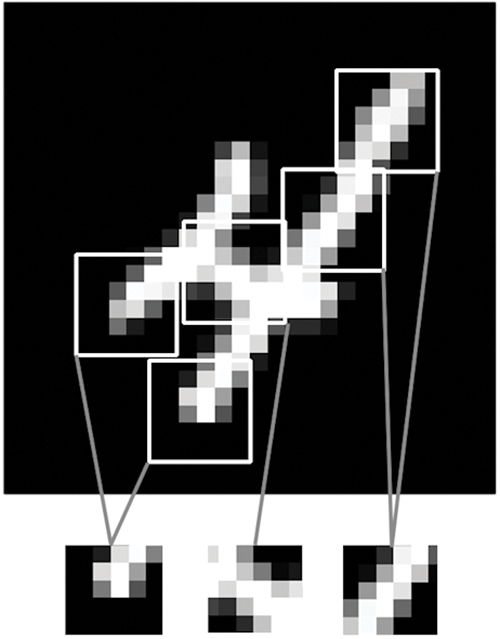
\includegraphics[width=\textwidth,height=0.7\textheight,keepaspectratio]{../../images/ch08/local_patterns.b72668dd.jpg}
            \caption{Local Patterns vs Global Patterns}
        \end{figure}
    \end{columns}
\end{frame}

\begin{frame}{Hệ thống Phân cấp Thị giác (Visual Hierarchy)}
    \begin{columns}
        \column{0.5\textwidth}
        \begin{itemize}
            \item CNN học theo một hệ thống phân cấp tự nhiên:
            \item \textbf{Lớp đầu tiên:} Học các đặc trưng đơn giản (Cạnh, Góc).
            \item \textbf{Lớp giữa:} Ghép các cạnh thành bộ phận (Mắt, Mũi, Lưỡi).
            \item \textbf{Lớp cuối:} Tổng hợp thành vật thể hoàn chỉnh (Con mèo, Con chó).
            \item Điều này giống hệt cách vỏ não thị giác (Visual Cortex) của con người hoạt động.
        \end{itemize}
        
        \column{0.5\textwidth}
        \begin{figure}
            \centering
            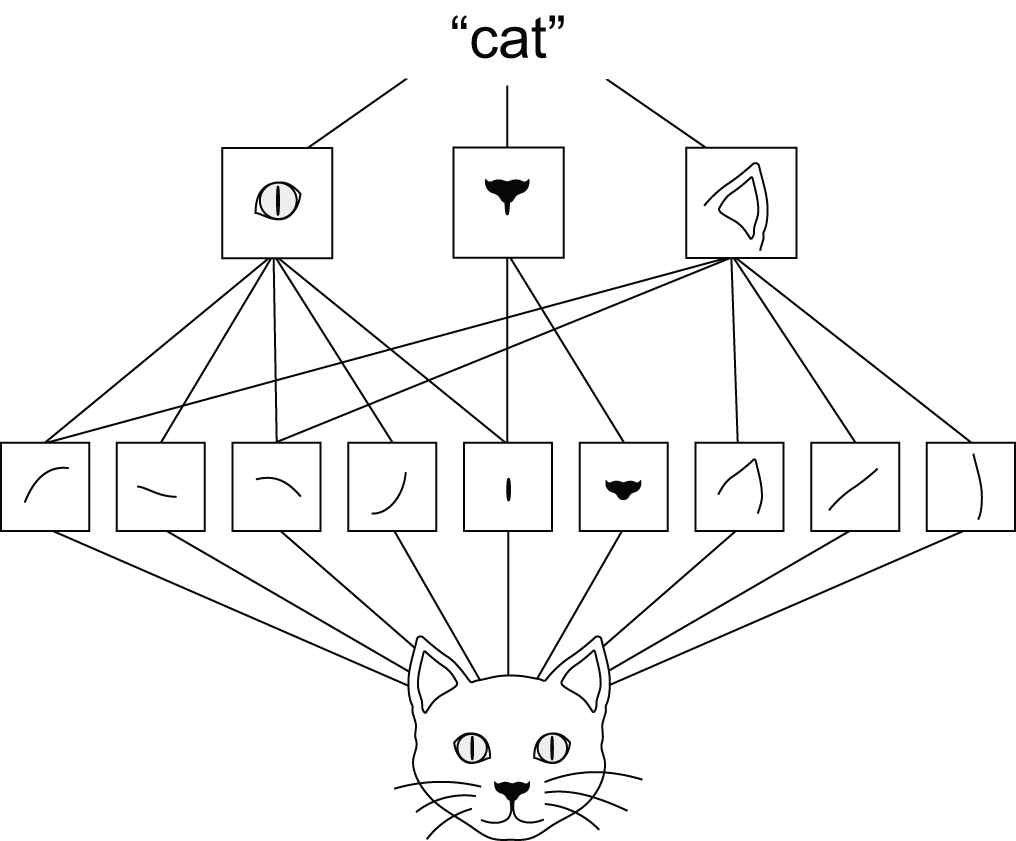
\includegraphics[width=\textwidth,height=0.7\textheight,keepaspectratio]{../../images/ch08/visual_hierarchy_hires.40ec558e.png}
            \caption{Sự kết hợp các đặc trưng bậc thấp thành bậc cao}
        \end{figure}
    \end{columns}
\end{frame}

\begin{frame}[fragile]{Mạng CNN cơ bản: Mã nguồn}
Cấu trúc một mạng phân loại ảnh đơn giản bao gồm việc xen kẽ các lớp \texttt{Conv2D} và \texttt{MaxPooling2D}.

\begin{lstlisting}[language=Python, basicstyle=\ttfamily\scriptsize]
import keras
from keras import layers

inputs = keras.Input(shape=(28, 28, 1))
x = layers.Conv2D(filters=64, kernel_size=3, activation="relu")(inputs)
x = layers.MaxPooling2D(pool_size=2)(x)
x = layers.Conv2D(filters=128, kernel_size=3, activation="relu")(x)
x = layers.MaxPooling2D(pool_size=2)(x)
x = layers.Conv2D(filters=256, kernel_size=3, activation="relu")(x)
x = layers.GlobalAveragePooling2D()(x)
outputs = layers.Dense(10, activation="softmax")(x)

model = keras.Model(inputs=inputs, outputs=outputs)
\end{lstlisting}
\end{frame}

\begin{frame}[fragile]{Kiểm tra quá trình nén không gian (Model Summary)}
Kích thước không gian (chiều rộng $\times$ chiều cao) giảm dần, trong khi chiều sâu (số kênh) tăng dần.

\begin{lstlisting}[language=Python, basicstyle=\ttfamily\tiny]
>>> model.summary()
Model: "functional"
...
Layer (type)                      Output Shape             Param #
===================================================================
input_layer (InputLayer)          (None, 28, 28, 1)        0
conv2d (Conv2D)                   (None, 26, 26, 64)       640
max_pooling2d (MaxPooling2D)      (None, 13, 13, 64)       0
conv2d_1 (Conv2D)                 (None, 11, 11, 128)      73856
max_pooling2d_1 (MaxPooling2D)    (None, 5, 5, 128)        0
conv2d_2 (Conv2D)                 (None, 3, 3, 256)        295168
global_average_pooling2d          (None, 256)              0
dense (Dense)                     (None, 10)               2570
...
\end{lstlisting}
\end{frame}

\begin{frame}{Toán học của Phép Tích chập (Dot Product)}
    \begin{columns}
        \column{0.5\textwidth}
        Toán tử Tích chập 2D được định nghĩa:
        \begin{equation}
            S(i,j) = (I * K)(i,j) = \sum_{m}\sum_{n} I(i-m, j-n) K(m,n)
        \end{equation}
        \begin{itemize}
            \item $I$: Ma trận ảnh đầu vào.
            \item $K$: Bộ lọc (Kernel / Filter).
            \item Bản chất là trượt bộ lọc $K$ trên toàn bộ ảnh và tính Tích vô hướng (Dot Product).
        \end{itemize}
        
        \column{0.5\textwidth}
        \begin{figure}
            \centering
            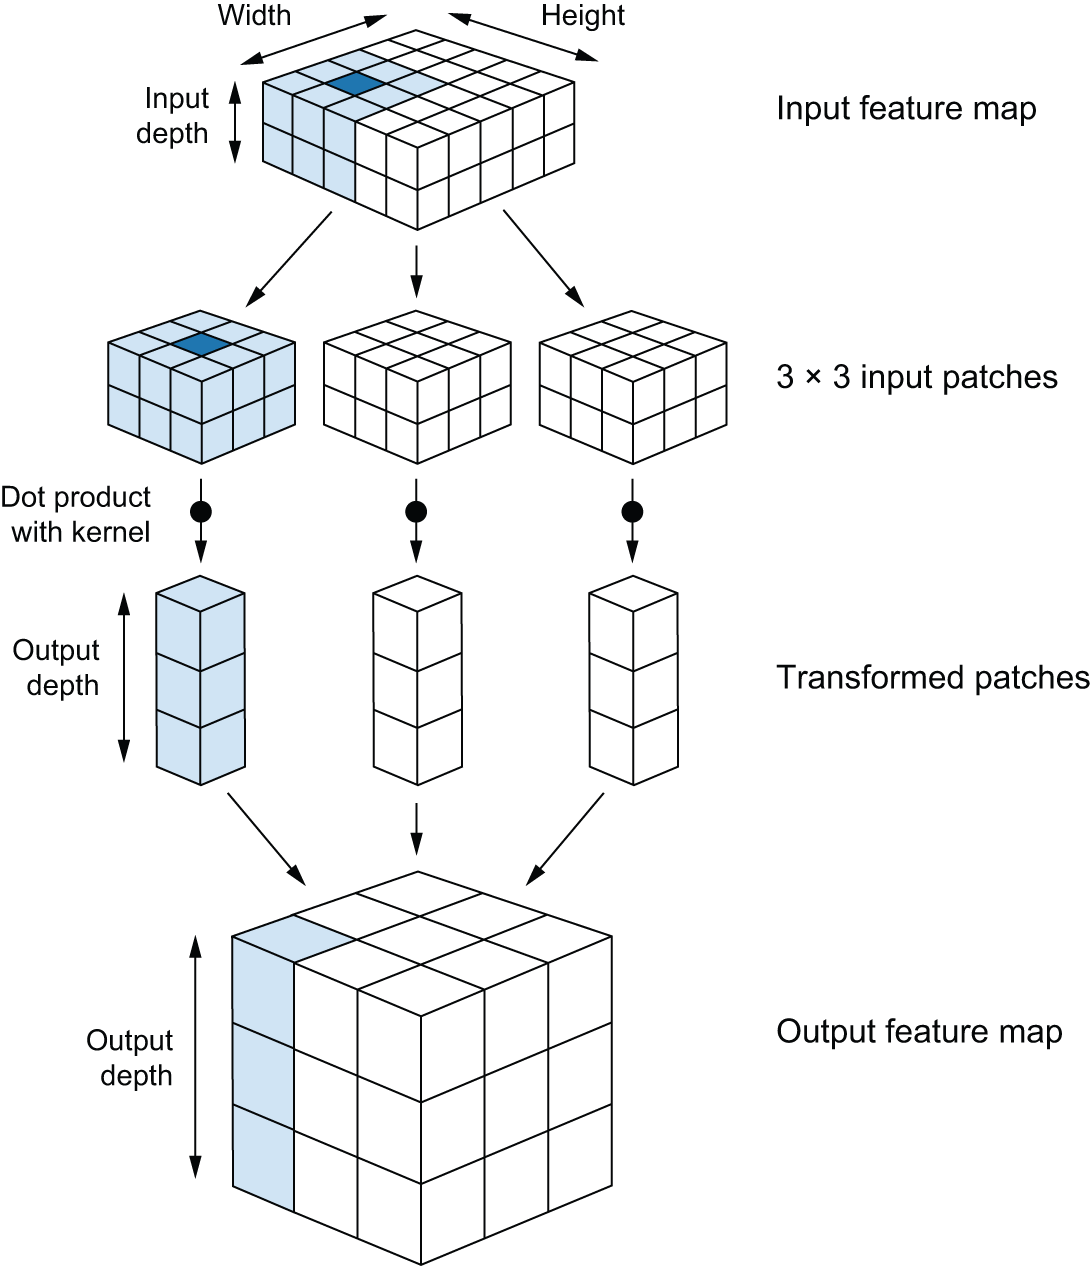
\includegraphics[width=\textwidth,height=0.7\textheight,keepaspectratio]{../../images/ch08/how_convolution_works.fb611af4.png}
            \caption{Phép trượt nhân chập cơ bản}
        \end{figure}
    \end{columns}
\end{frame}

\begin{frame}{Trích xuất Phân mảnh (Patches)}
    \begin{columns}
        \column{0.5\textwidth}
        \begin{itemize}
            \item Nếu có ảnh đầu vào kích thước $5 \times 5$, và sử dụng Bộ lọc kích thước $3 \times 3$.
            \item Bộ lọc sẽ cắt ra các \textbf{phân mảnh (patches)} có cùng kích thước $3 \times 3$.
            \item Khớp với mỗi phân mảnh, phép Tích vô hướng sẽ sinh ra duy nhất một con số (Scalar).
        \end{itemize}
        
        \column{0.5\textwidth}
        \begin{figure}
            \centering
            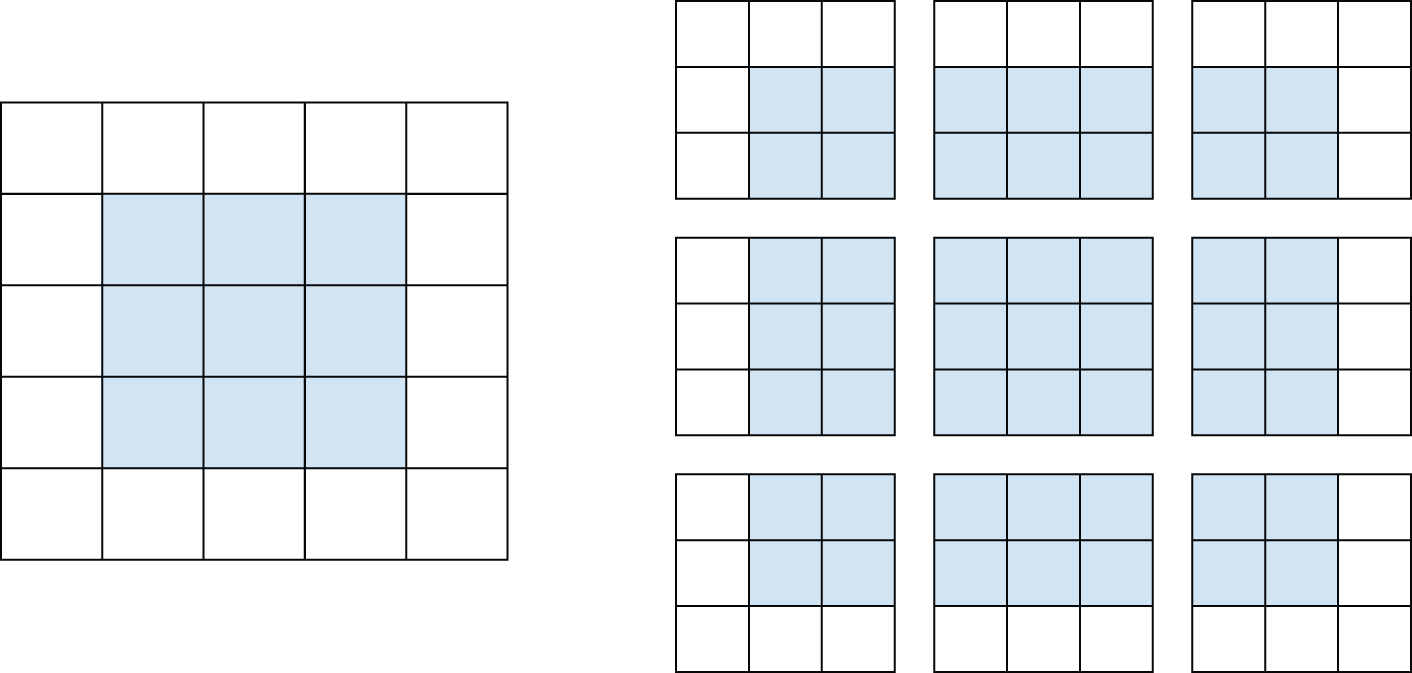
\includegraphics[width=\textwidth,height=0.7\textheight,keepaspectratio]{../../images/ch08/3x3_patches_in_5x5_input.3954b81b.png}
            \caption{Trích xuất các patches $3 \times 3$}
        \end{figure}
    \end{columns}
\end{frame}

\begin{frame}{Bản đồ Phản hồi (Response Map)}
    \begin{columns}
        \column{0.5\textwidth}
        \begin{itemize}
            \item Mỗi Bộ lọc (Filter) đại diện cho một "Khái niệm" (Vd: Khái niệm "có mắt mèo trong hình không?").
            \item Kết quả của quá trình tích chập tạo ra một \textbf{Bản đồ phản hồi (Response Map)}.
            \item Điểm nào sáng trên bản đồ nghĩa là Bộ lọc đã "nhìn thấy" mẫu mà nó đang tìm kiếm tại vị trí đó.
        \end{itemize}
        
        \column{0.5\textwidth}
        \begin{figure}
            \centering
            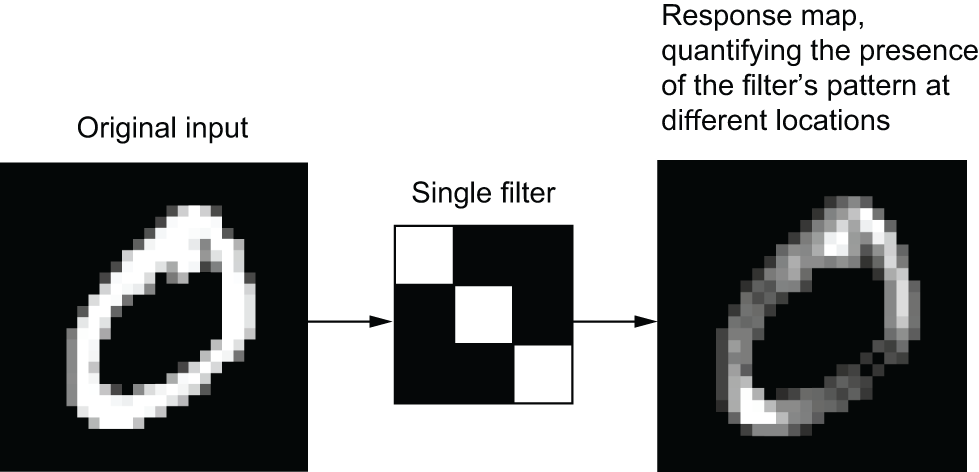
\includegraphics[width=\textwidth,height=0.7\textheight,keepaspectratio]{../../images/ch08/response_map_hires.ab2ee335.png}
            \caption{Một bản đồ phản hồi đặc trưng}
        \end{figure}
    \end{columns}
\end{frame}

\begin{frame}{Kỹ thuật Lấp đầy (Padding)}
    \begin{columns}
        \column{0.5\textwidth}
        \begin{itemize}
            \item Kích thước ảnh luôn bị \textbf{co hẹp lại} sau khi Tích chập (Từ $5 \times 5$ xuống $3 \times 3$).
            \item Lớp biên của ảnh gốc bị bỏ qua rất nhiều.
            \item \textbf{Padding:} Thêm các viền số 0 (Zero-padding) bao quanh ảnh để bảo toàn kích thước sau khi quét.
            \item Tham số Keras: \texttt{padding="same"} (Bảo toàn) hoặc \texttt{padding="valid"} (Không lấp đầy).
        \end{itemize}
        
        \column{0.5\textwidth}
        \begin{figure}
            \centering
            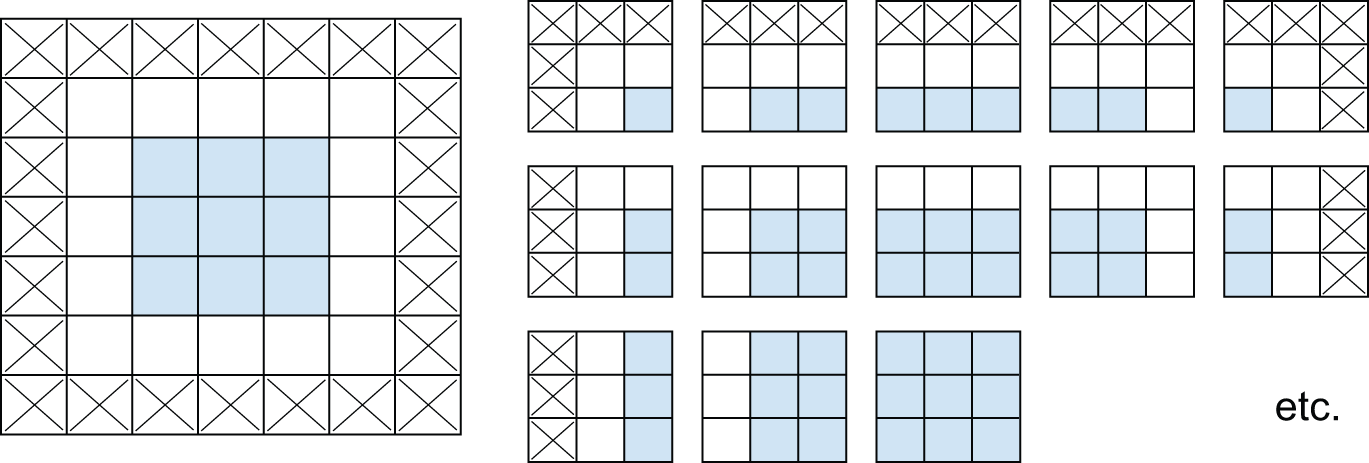
\includegraphics[width=\textwidth,height=0.7\textheight,keepaspectratio]{../../images/ch08/padding_of_5x5_input.fb864a53.png}
            \caption{Minh họa Zero Padding}
        \end{figure}
    \end{columns}
\end{frame}

\begin{frame}{Bước nhảy (Strides)}
    \begin{columns}
        \column{0.5\textwidth}
        \begin{itemize}
            \item \textbf{Stride:} Khoảng cách (số pixel) mà Bộ lọc trượt đi sau mỗi nhịp.
            \item Mặc định là \texttt{strides=1}.
            \item Nếu \texttt{strides=2}, bộ lọc sẽ nhảy cóc qua 1 pixel. Kích thước bản đồ đầu ra sẽ giảm đi chính xác một nửa (Downsampling).
            \item \textit{Tuy nhiên, trong thực tế ta thường dùng MaxPooling để giảm kích thước thay vì Strides.}
        \end{itemize}
        
        \column{0.5\textwidth}
        \begin{figure}
            \centering
            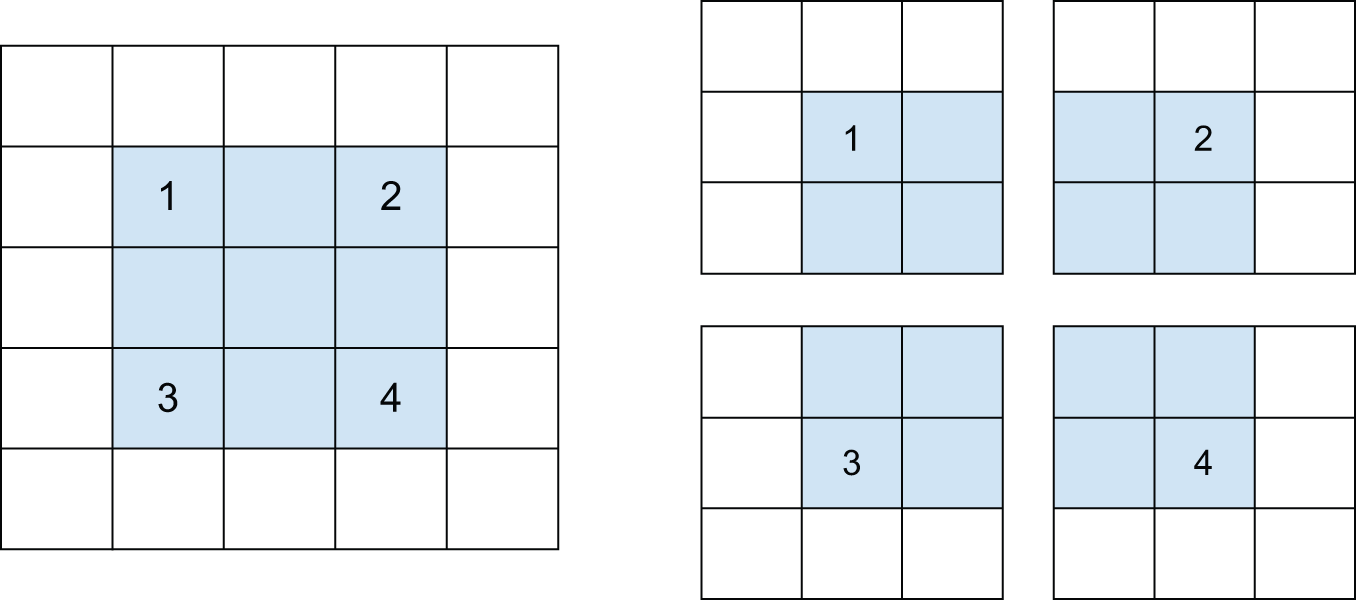
\includegraphics[width=\textwidth,height=0.7\textheight,keepaspectratio]{../../images/ch08/strides.78c3a935.png}
            \caption{Bộ lọc trượt với Strides bằng 2}
        \end{figure}
    \end{columns}
\end{frame}

\section{2. Thực hành: Bài toán Phân loại Chó \& Mèo}

\begin{frame}{Tập Dữ liệu Kaggle Dogs vs Cats}
    \begin{columns}
        \column{0.5\textwidth}
        \begin{itemize}
            \item Bài toán thi đấu nổi tiếng năm 2013 trên Kaggle.
            \item Cung cấp 25,000 ảnh chó và mèo nhiều kích cỡ, màu sắc, bối cảnh.
            \item Ta sẽ trích xuất ra một tập con siêu nhỏ (Chỉ 2,000 ảnh cho Training) để giả lập kịch bản \textbf{thiếu dữ liệu} rất phổ biến trong doanh nghiệp.
        \end{itemize}
        
        \column{0.5\textwidth}
        \begin{figure}
            \centering
            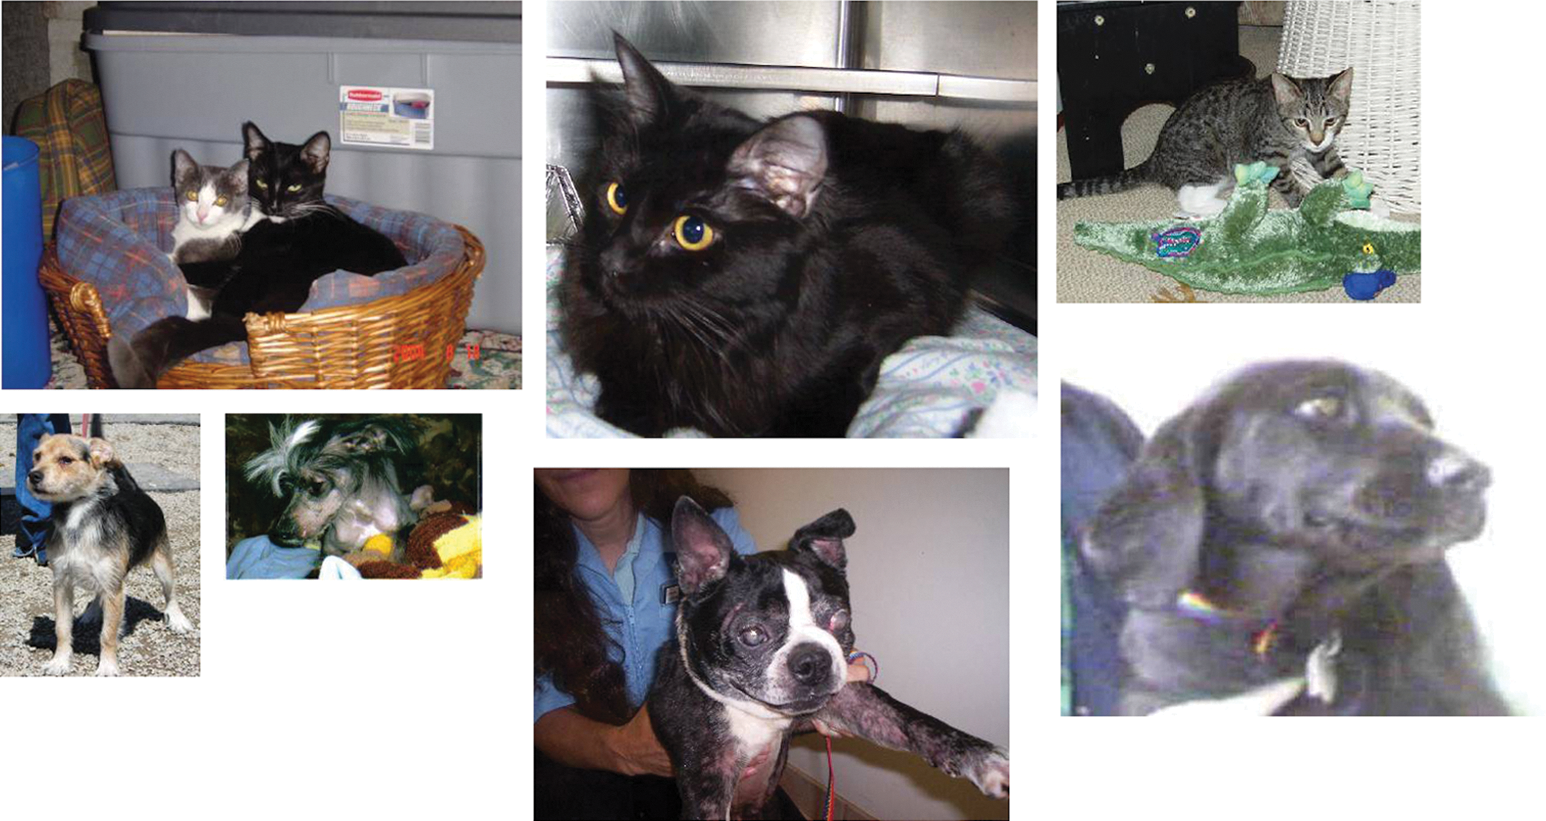
\includegraphics[width=\textwidth,height=0.7\textheight,keepaspectratio]{../../images/ch08/dog_and_cat_samples.d2409a95.png}
            \caption{Mẫu ảnh từ bộ dữ liệu}
        \end{figure}
    \end{columns}
\end{frame}

\begin{frame}[fragile]{Tiền xử lý ảnh với Keras: \texttt{image\_dataset\_from\_directory}}
Với những dữ liệu lớn, việc đọc tất cả vào RAM là bất khả thi. \texttt{image\_dataset\_from\_directory} tạo một \textbf{Data Generator} lấy ảnh trực tiếp từ ổ cứng theo từng lô.

\begin{lstlisting}[language=Python, basicstyle=\ttfamily\scriptsize]
from keras.utils import image_dataset_from_directory

train_dataset = image_dataset_from_directory(
    "dogs_vs_cats_small/train",
    image_size=(180, 180),
    batch_size=32
)

validation_dataset = image_dataset_from_directory(
    "dogs_vs_cats_small/validation",
    image_size=(180, 180),
    batch_size=32
)
\end{lstlisting}
\end{frame}

\begin{frame}{Huấn luyện CNN cơ bản (Từ con số 0)}
    \begin{columns}
        \column{0.5\textwidth}
        \begin{itemize}
            \item Thiết kế mạng với 4 khối \texttt{Conv2D + MaxPooling2D}.
            \item Kết quả: Validation Accuracy đạt khoảng 70-75\% rồi chững lại.
            \item Khoảng cách giữa đường Train (Xanh) và Validation (Đứt nét) nới rộng nhanh chóng $\rightarrow$ \textbf{Dấu hiệu Overfitting điển hình.}
        \end{itemize}
        
        \column{0.5\textwidth}
        \begin{figure}
            \centering
            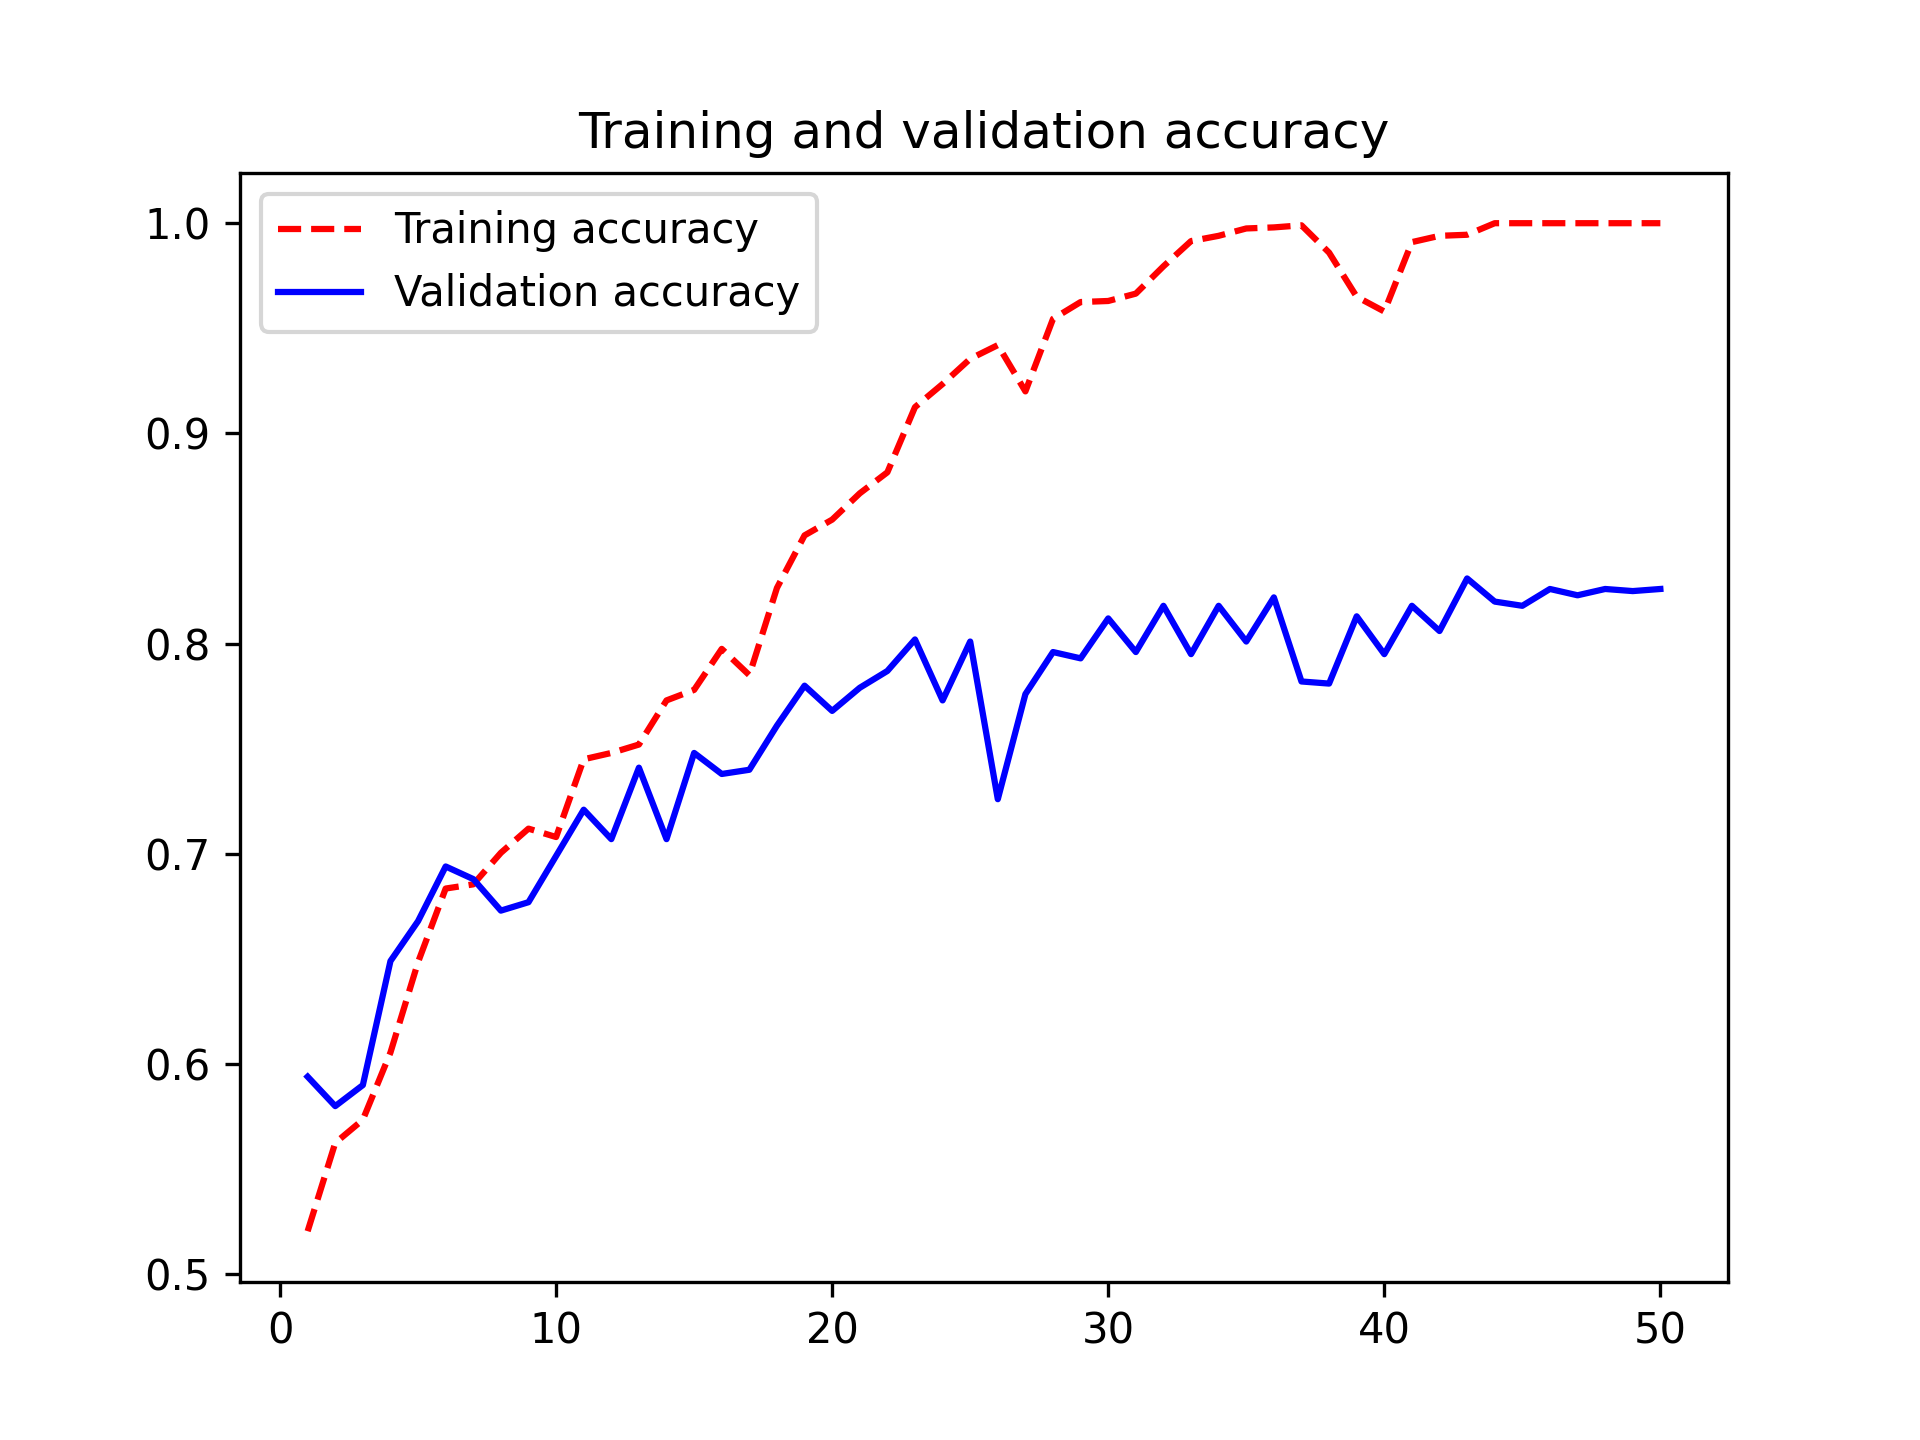
\includegraphics[width=\textwidth,height=0.5\textheight,keepaspectratio]{../../images/ch08/cats-and-dogs-1-training-and-validation-acc.c0b7aa87.png}
            \caption{Accuracy Mô hình cơ bản}
        \end{figure}
    \end{columns}
\end{frame}

\begin{frame}{Phân tích hàm Loss cơ bản}
    \begin{columns}
        \column{0.5\textwidth}
        \begin{itemize}
            \item Hàm mất mát Training liên tục giảm tiến về 0. Mô hình đang "thuộc lòng" (Memorizing) dữ liệu học.
            \item Hàm mất mát Validation không thể giảm xuống dưới ngưỡng 0.8 và bắt đầu bật tăng ngược trở lại sau Epoch 10.
            \item \textbf{Kết luận:} Do dữ liệu huấn luyện quá ít (2000 ảnh), mạng CNN không thể khái quát hóa. Ta cần kỹ thuật mạnh hơn.
        \end{itemize}
        
        \column{0.5\textwidth}
        \begin{figure}
            \centering
            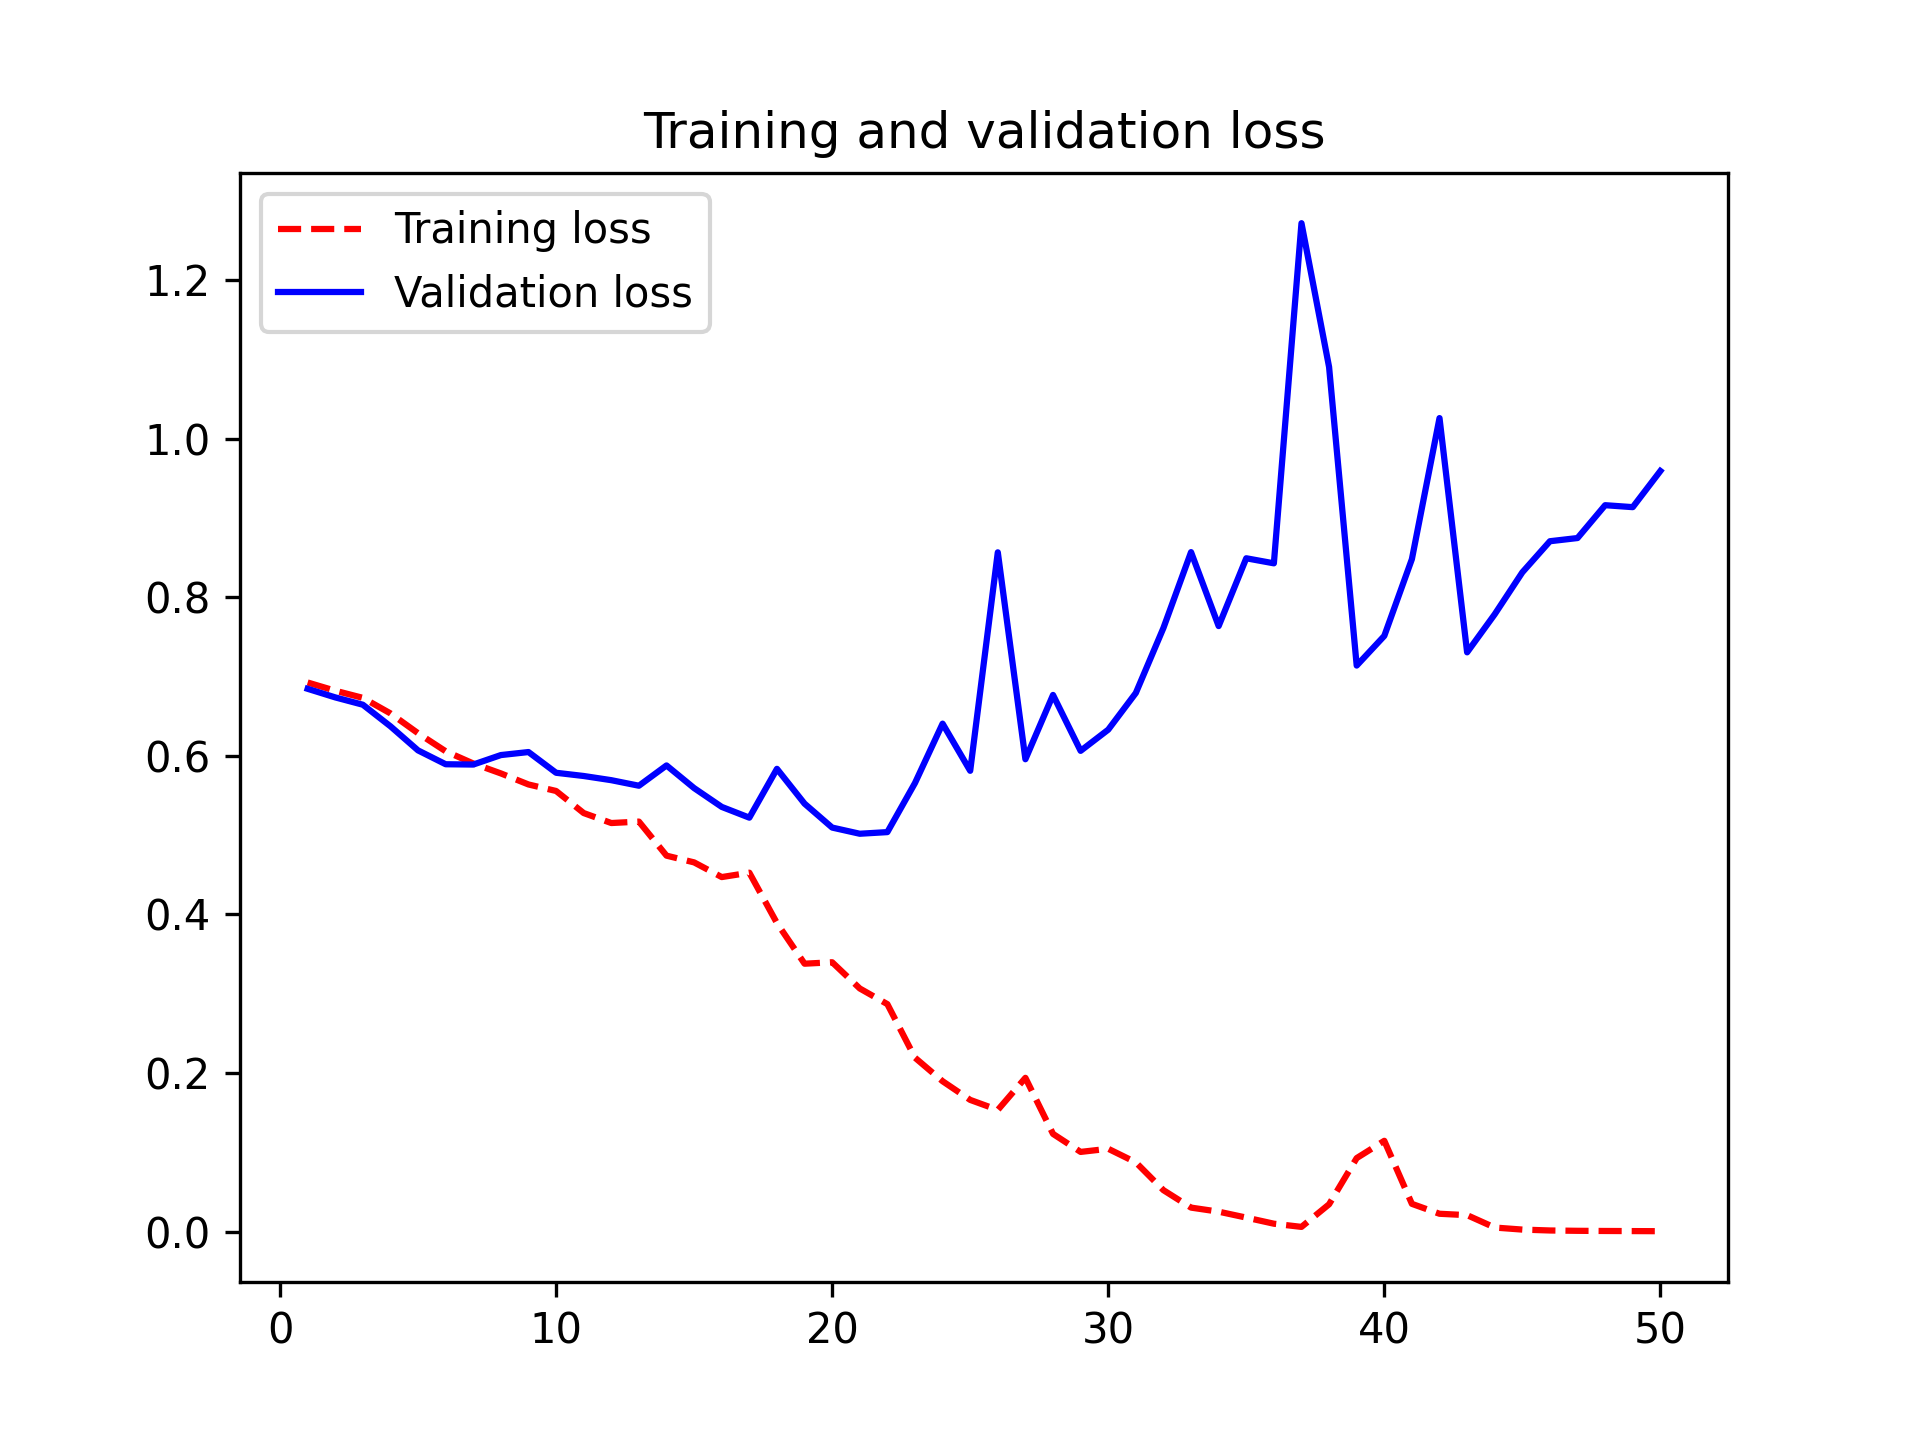
\includegraphics[width=\textwidth,height=0.5\textheight,keepaspectratio]{../../images/ch08/cats-and-dogs-1-training-and-validation-loss.cbe4e0a3.png}
            \caption{Loss Mô hình cơ bản}
        \end{figure}
    \end{columns}
\end{frame}

\section{3. Chống Overfitting bằng Data Augmentation}

\begin{frame}{Kỹ thuật Tăng cường Dữ liệu (Data Augmentation)}
    \begin{columns}
        \column{0.5\textwidth}
        \begin{itemize}
            \item Không có thêm dữ liệu? Hãy \textbf{tự tạo ra dữ liệu mới} từ dữ liệu cũ!
            \item Áp dụng các phép biến đổi ngẫu nhiên: Xoay (Rotation), Dịch chuyển (Translation), Thu phóng (Zoom), Lật ngang (Horizontal Flip).
            \item Mô hình sẽ không bao giờ nhìn thấy cùng một bức ảnh 2 lần, buộc nó phải học các đặc trưng \textit{bất biến}.
        \end{itemize}
        
        \column{0.5\textwidth}
        \begin{figure}
            \centering
            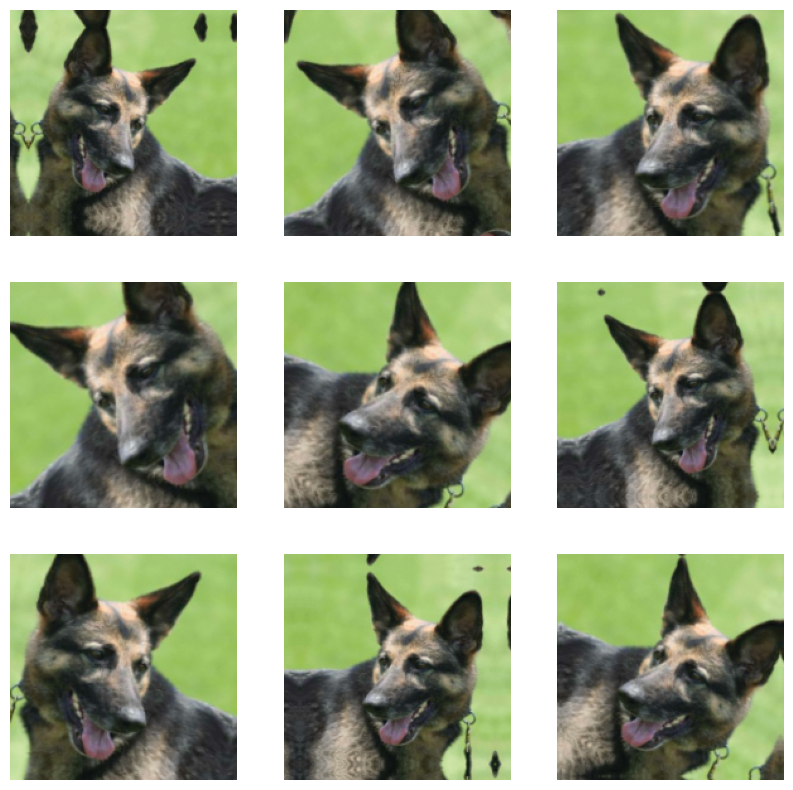
\includegraphics[width=\textwidth,height=0.7\textheight,keepaspectratio]{../../images/ch08/augmented_data.63e74cdb.png}
            \caption{Cùng một con mèo nhưng sinh ra nhiều biến thể}
        \end{figure}
    \end{columns}
\end{frame}

\begin{frame}[fragile]{Data Augmentation: Mã nguồn}
Keras cung cấp sẵn các Layer tăng cường dữ liệu. Các lớp này có thể được gắn thẳng vào mô hình.

\begin{lstlisting}[language=Python, basicstyle=\ttfamily\scriptsize]
data_augmentation = keras.Sequential(
    [
        layers.RandomFlip("horizontal"),
        layers.RandomRotation(0.1),
        layers.RandomZoom(0.2),
    ]
)

# Insert augmentation layer before the main ConvNets
inputs = keras.Input(shape=(180, 180, 3))
x = data_augmentation(inputs)
x = layers.Rescaling(1./255)(x)
x = layers.Conv2D(filters=32, kernel_size=3, activation="relu")(x)
# ... Add more Convolutional Blocks ...
\end{lstlisting}
\textit{Lưu ý: Data Augmentation tự động bị Vô hiệu hóa (Deactivated) trong quá trình Testing / Validation.}
\end{frame}

\begin{frame}{Đánh giá Accuracy sau Augmentation}
    \begin{columns}
        \column{0.5\textwidth}
        \begin{itemize}
            \item Validation Accuracy đã tăng từ 70\% lên \textbf{hơn 80\%}.
            \item Quan trọng hơn: Đường Validation (Đứt nét) bám sát đường Training (Xanh).
            \item Mô hình hoàn toàn không còn hiện tượng Overfitting, và chúng ta có thể tiếp tục huấn luyện lâu hơn.
        \end{itemize}
        
        \column{0.5\textwidth}
        \begin{figure}
            \centering
            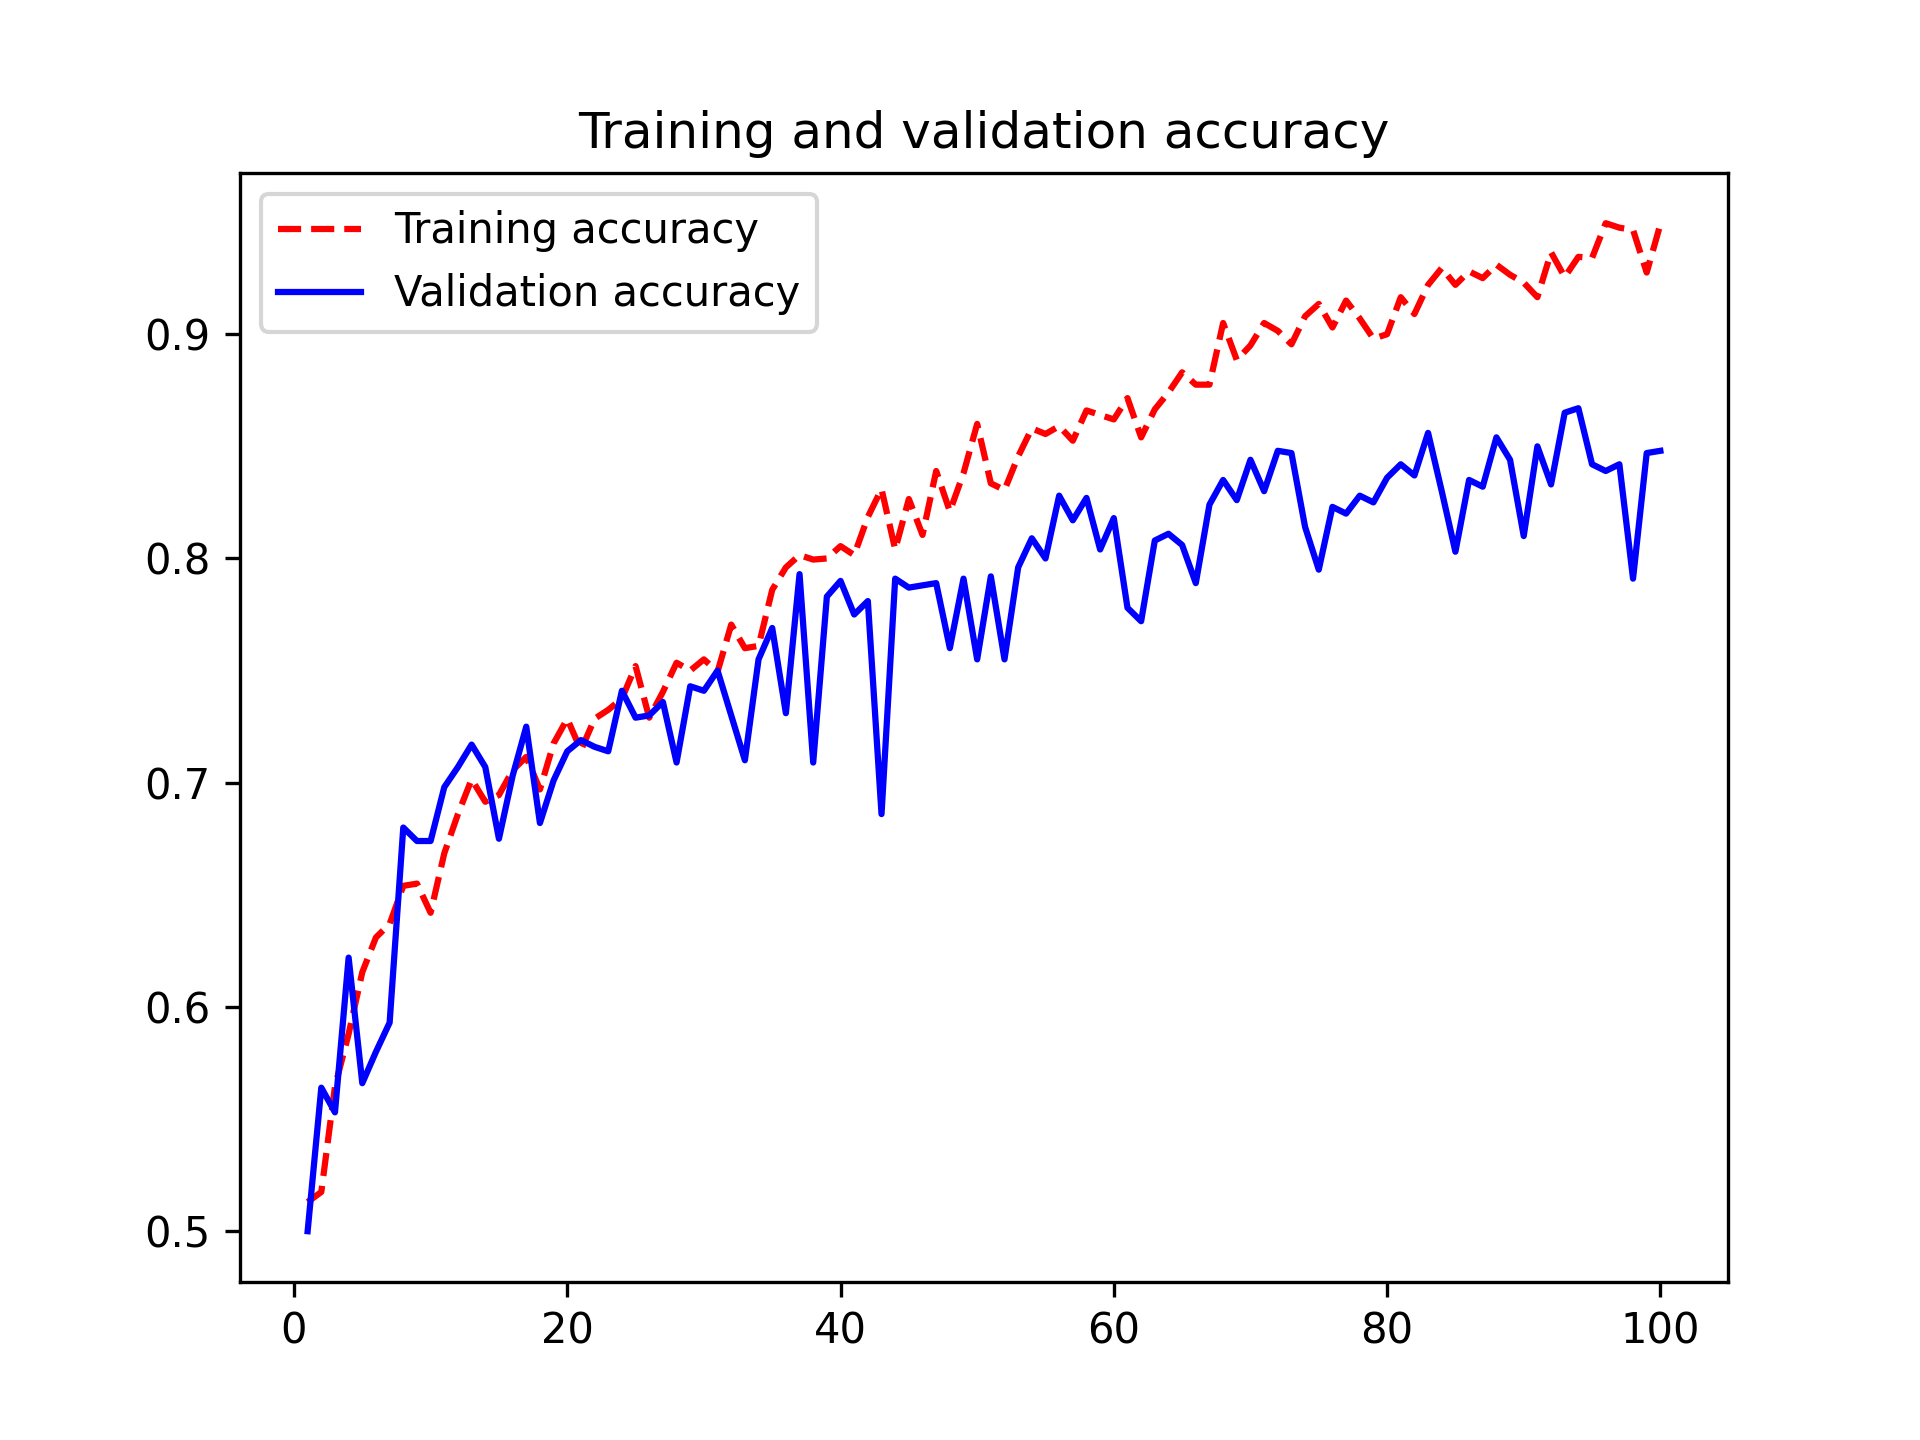
\includegraphics[width=\textwidth,height=0.5\textheight,keepaspectratio]{../../images/ch08/cats-and-dogs-1-training-and-validation-da-acc.95f4446c.png}
            \caption{Accuracy có Data Augmentation}
        \end{figure}
    \end{columns}
\end{frame}

\begin{frame}{Đánh giá Loss sau Augmentation}
    \begin{columns}
        \column{0.5\textwidth}
        \begin{itemize}
            \item Đồ thị Loss không còn bị nảy ngược lên như trước.
            \item Kỹ thuật Augmentation được tính toán song song trên CPU/GPU qua hàm \texttt{tf.data} pipeline mà không làm chậm quá trình Train.
            \item \textbf{Giới hạn:} Ta vẫn đang bị kẹt ở mốc 82\%. Để vượt ngưỡng này, ta cần sức mạnh từ Transfer Learning.
        \end{itemize}
        
        \column{0.5\textwidth}
        \begin{figure}
            \centering
            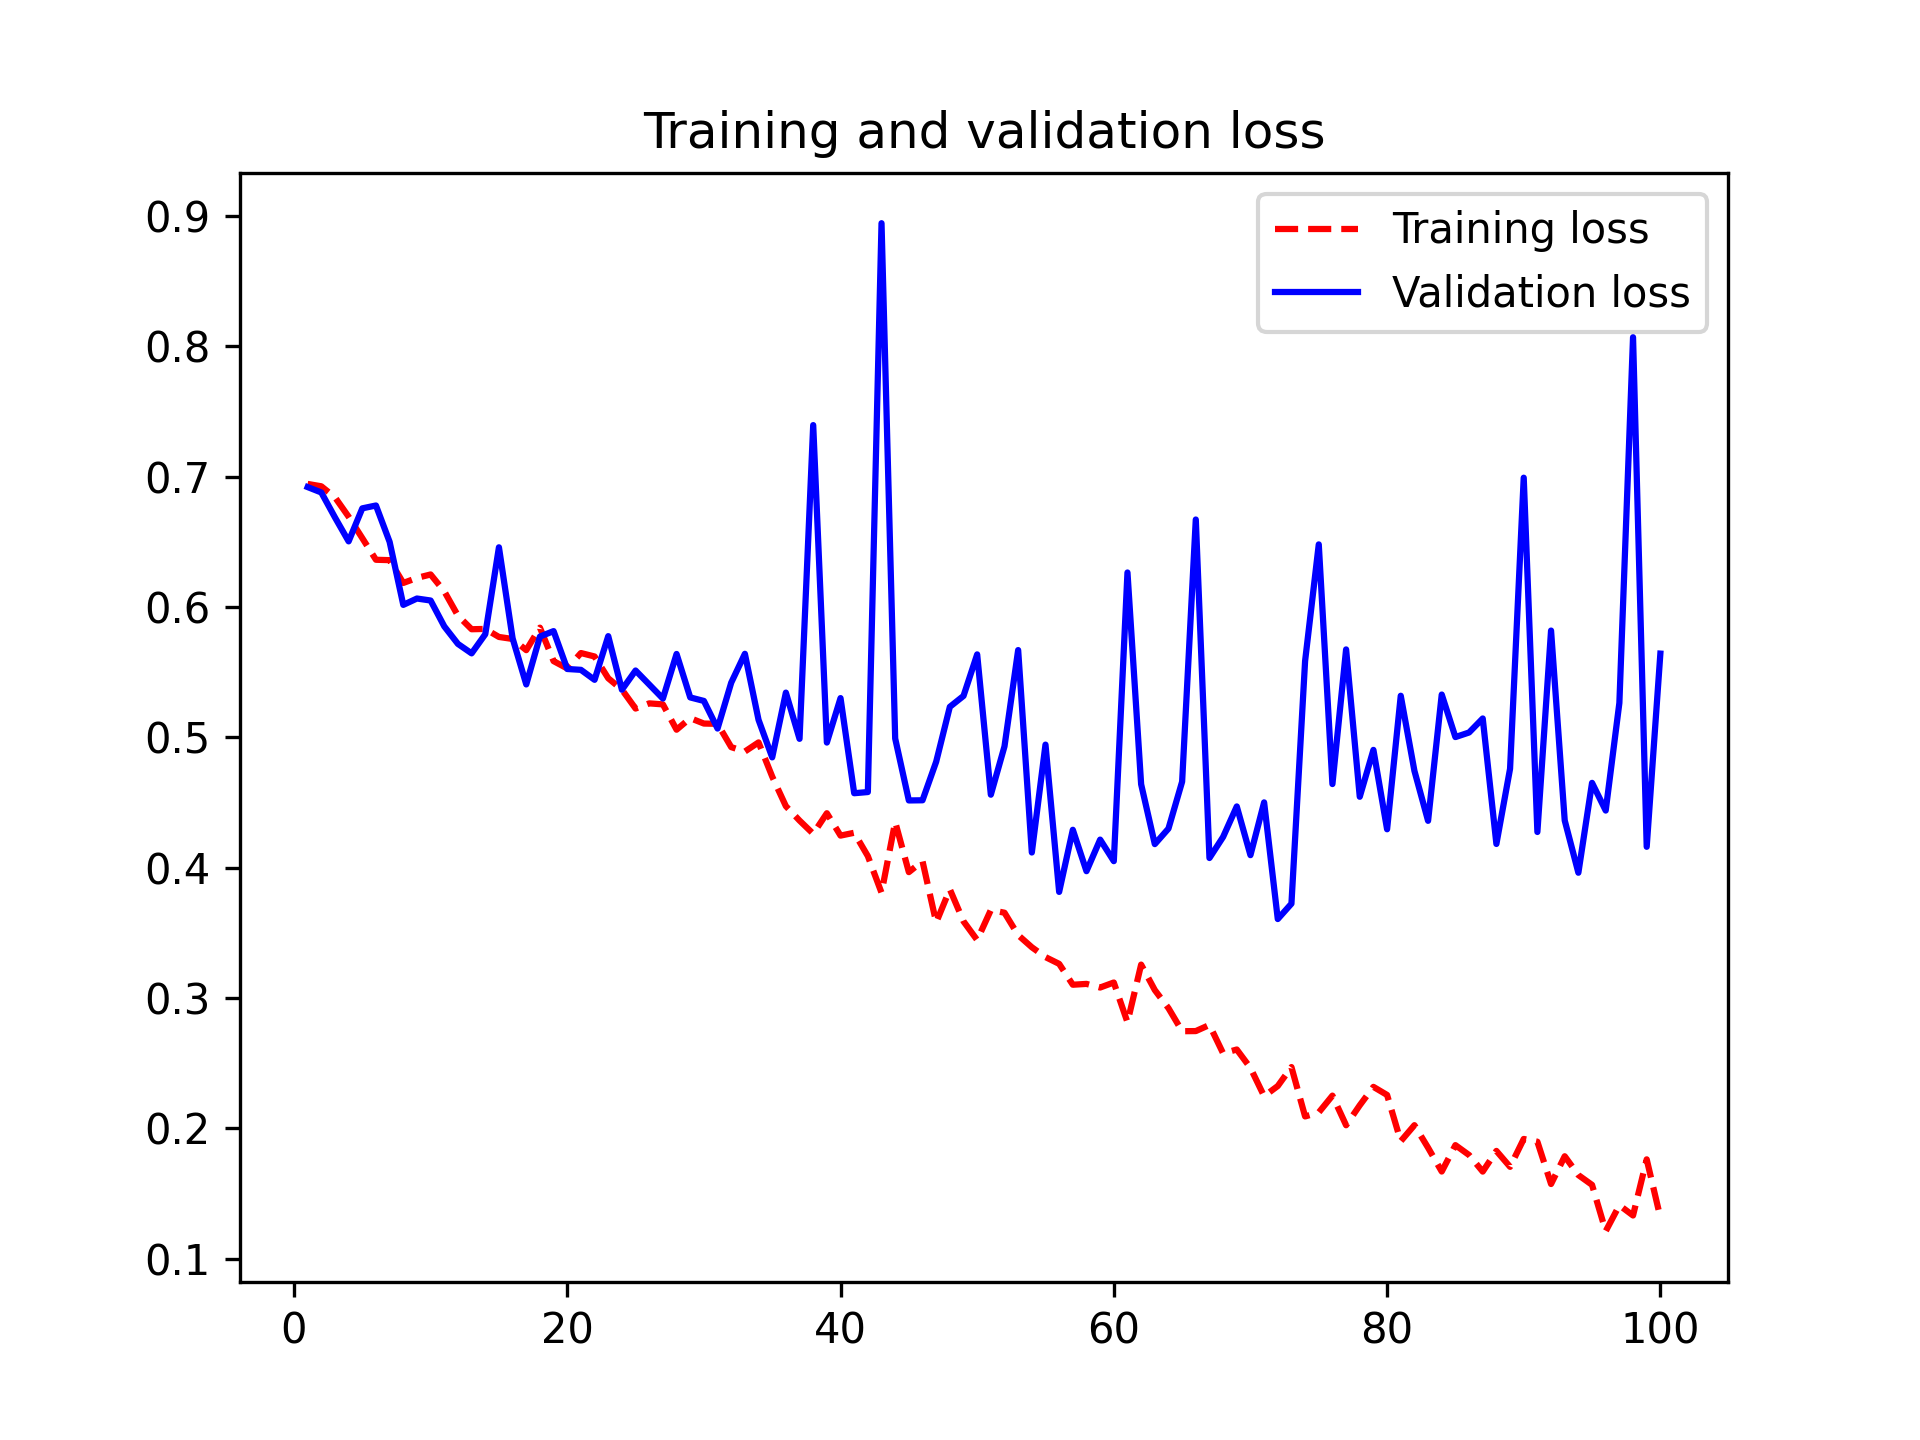
\includegraphics[width=\textwidth,height=0.5\textheight,keepaspectratio]{../../images/ch08/cats-and-dogs-1-training-and-validation-da-loss.fb77981b.png}
            \caption{Loss có Data Augmentation}
        \end{figure}
    \end{columns}
\end{frame}

\section{4. Chuyển giao Học tập (Transfer Learning)}

\begin{frame}{Trích xuất Đặc trưng (Feature Extraction)}
    \begin{columns}
        \column{0.5\textwidth}
        \begin{itemize}
            \item \textbf{Khái niệm:} Tái sử dụng một mô hình cực lớn (VGG16) đã được huấn luyện trên 1.4 triệu bức ảnh của ImageNet.
            \item \textbf{Kiến trúc:} Giữ nguyên Khối Tích chập (Convolutional Base) của VGG16.
            \item Cắt bỏ phần đầu Phân loại (Fully Connected Classifier) cũ của VGG16, và \textbf{Gắn lõi Phân loại mới} của chúng ta vào.
        \end{itemize}
        
        \column{0.5\textwidth}
        \begin{figure}
            \centering
            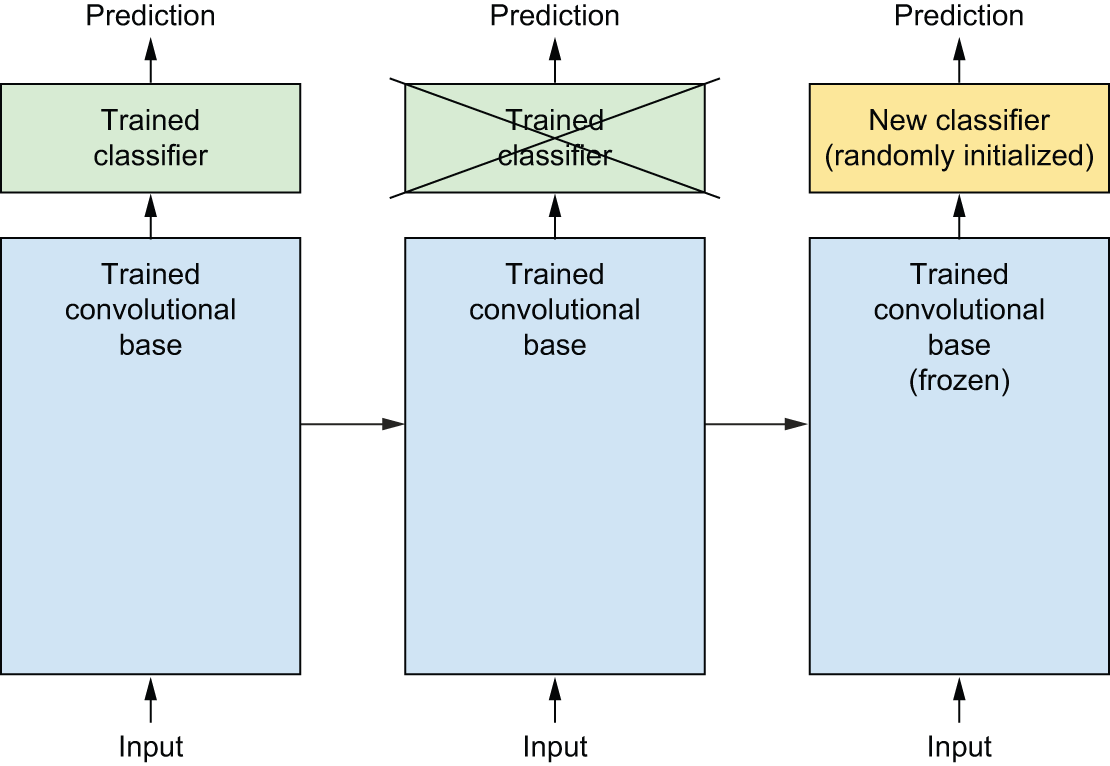
\includegraphics[width=\textwidth,height=0.7\textheight,keepaspectratio]{../../images/ch08/swapping_fc_classifier.6e525b7a.png}
            \caption{Thay thế bộ phân loại (Swapping FC)}
        \end{figure}
    \end{columns}
\end{frame}

\begin{frame}[fragile]{Feature Extraction: Mã nguồn (Sử dụng VGG16)}
Khởi tạo mô hình VGG16, sau đó "Đóng băng" (Freeze) toàn bộ trọng số của Base.

\begin{lstlisting}[language=Python, basicstyle=\ttfamily\scriptsize]
# Load pre-trained model without the top dense layers (include_top=False)
conv_base = keras.applications.vgg16.VGG16(
    weights="imagenet",
    include_top=False,
    input_shape=(180, 180, 3)
)

# Freeze the base!
conv_base.trainable = False

# Attach our custom classifier
inputs = keras.Input(shape=(180, 180, 3))
x = conv_base(inputs)
x = layers.Flatten()(x)
x = layers.Dense(256, activation="relu")(x)
x = layers.Dropout(0.5)(x)
outputs = layers.Dense(1, activation="sigmoid")(x)
model = keras.Model(inputs, outputs)
\end{lstlisting}
\end{frame}

\begin{frame}{Accuracy với Feature Extraction Cơ bản}
    \begin{columns}
        \column{0.5\textwidth}
        \begin{itemize}
            \item Bằng cách đóng băng (Freeze) VGG16 Base, ta chỉ huấn luyện lớp \texttt{Dense} mới thêm vào.
            \item Kết quả đáng kinh ngạc: Validation Accuracy vọt lên \textbf{90\%}.
            \item Sự mạnh mẽ của ImageNet đã giúp trích xuất các đặc trưng mắt mèo/mũi chó cực kỳ tinh xảo.
        \end{itemize}
        
        \column{0.5\textwidth}
        \begin{figure}
            \centering
            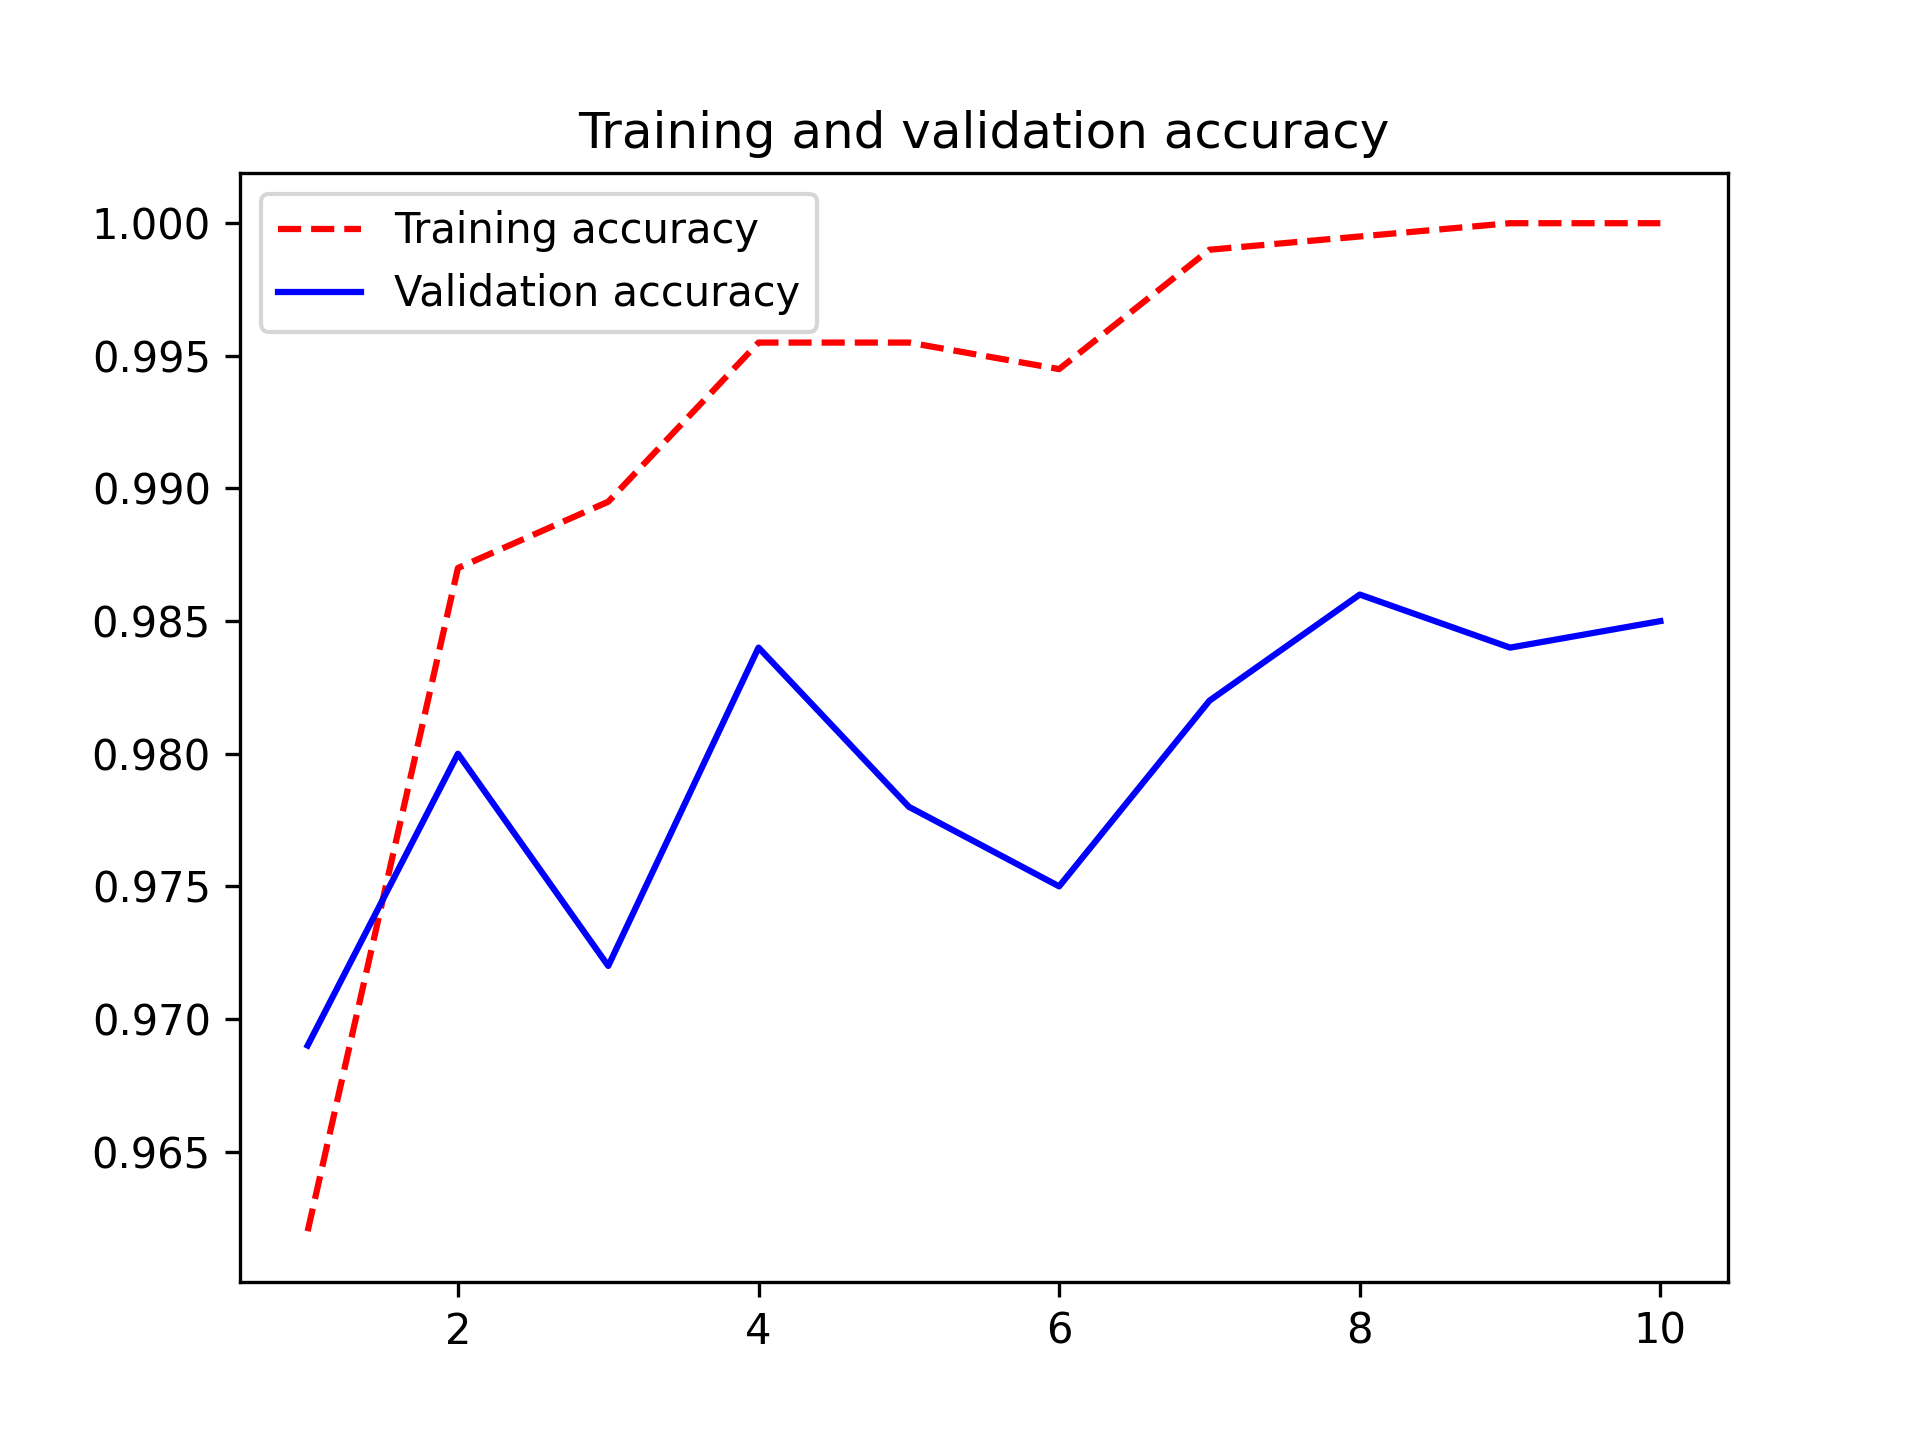
\includegraphics[width=\textwidth,height=0.5\textheight,keepaspectratio]{../../images/ch08/training-and-validation-fe-acc.2e8c417c.png}
            \caption{Accuracy Feature Extraction}
        \end{figure}
    \end{columns}
\end{frame}

\begin{frame}{Loss với Feature Extraction Cơ bản}
    \begin{columns}
        \column{0.5\textwidth}
        \begin{itemize}
            \item Tuy nhiên, vì tốc độ học quá nhanh, đồ thị Loss lại tiếp tục báo hiệu \textbf{Overfitting cực kỳ nặng} ngay từ Epoch thứ 5.
            \item Tại sao? Vì ta chưa áp dụng Data Augmentation cho quy trình này.
        \end{itemize}
        
        \column{0.5\textwidth}
        \begin{figure}
            \centering
            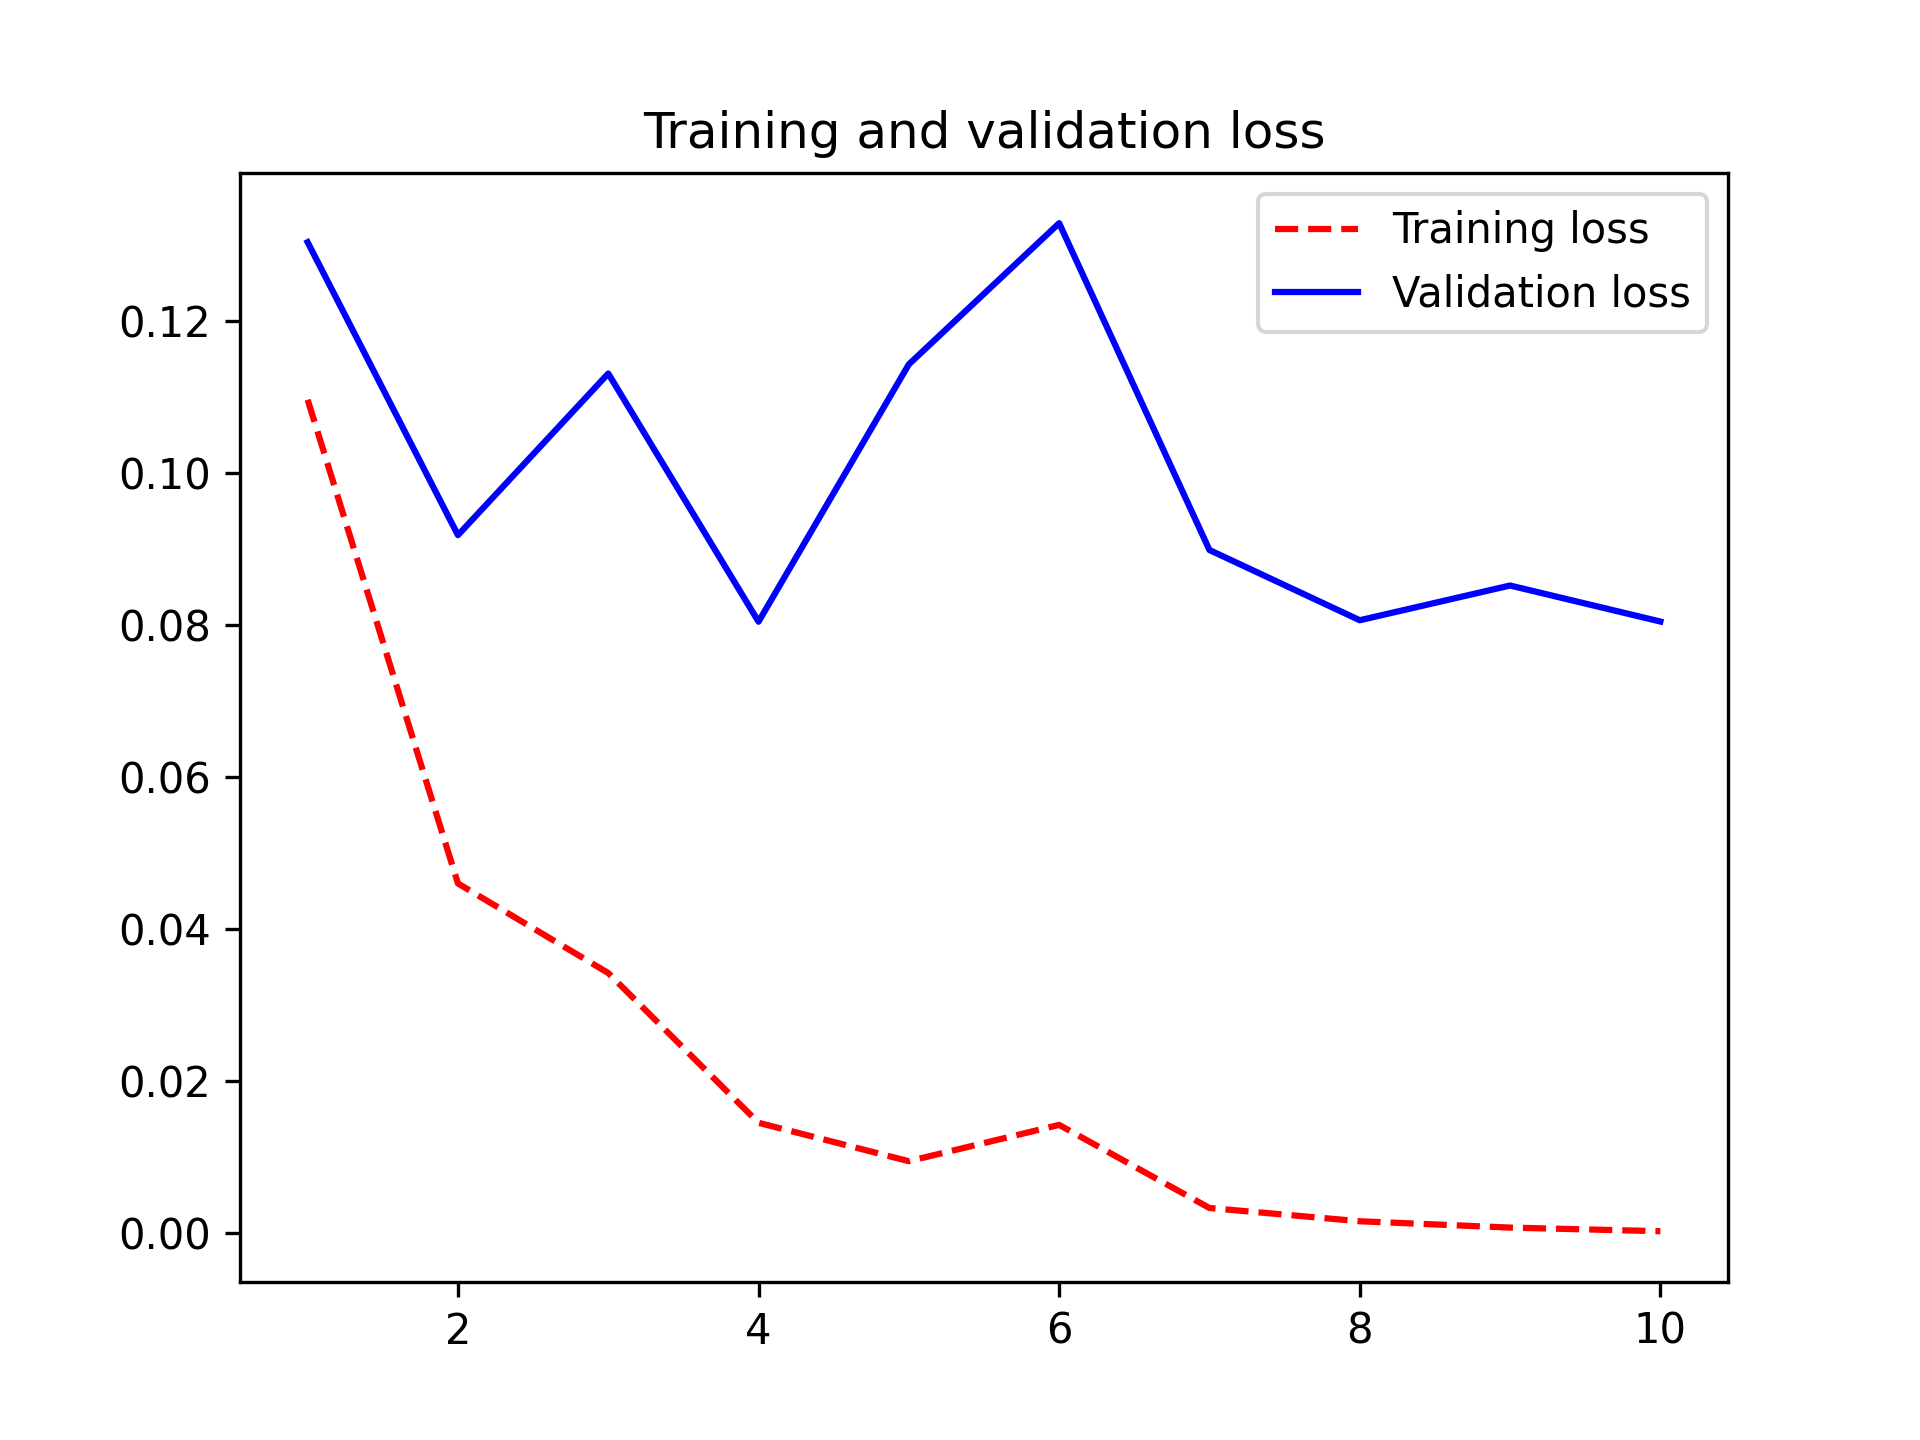
\includegraphics[width=\textwidth,height=0.5\textheight,keepaspectratio]{../../images/ch08/training-and-validation-fe-loss.49f7ffe0.png}
            \caption{Loss Feature Extraction (Bị Overfitting)}
        \end{figure}
    \end{columns}
\end{frame}

\begin{frame}[fragile]{Mô hình Liên hoàn: Feature Extraction + Data Augmentation}
Để giải quyết bài toán Overfitting, ta kết hợp Data Augmentation vào chuỗi tính toán.

\begin{lstlisting}[language=Python, basicstyle=\ttfamily\scriptsize]
inputs = keras.Input(shape=(180, 180, 3))
# 1. Apply Augmentation
x = data_augmentation(inputs)
# 2. Preprocess specifically for VGG16
x = keras.applications.vgg16.preprocess_input(x)
# 3. Extract features via Frozen Base
x = conv_base(x)
# 4. Custom classifier
x = layers.Flatten()(x)
x = layers.Dense(256)(x)
x = layers.Dropout(0.5)(x)
outputs = layers.Dense(1, activation="sigmoid")(x)
model = keras.Model(inputs, outputs)
\end{lstlisting}
\textit{Đây là kỹ thuật yêu cầu GPU mạnh vì phải chạy forward-pass qua toàn bộ Base nhiều lần.}
\end{frame}

\begin{frame}{Accuracy với Feature Extraction + Data Augmentation}
    \begin{columns}
        \column{0.5\textwidth}
        \begin{itemize}
            \item Ta thiết lập một kiến trúc liên hoàn: Lớp Augmentation $\rightarrow$ VGG16 Base (Đóng băng) $\rightarrow$ Lớp \texttt{Dense} (Huấn luyện).
            \item Kết quả: \textbf{Mượt mà hoàn hảo}. Validation bám sát Training và không còn Overfitting. Đạt mốc \textbf{96\%}.
        \end{itemize}
        
        \column{0.5\textwidth}
        \begin{figure}
            \centering
            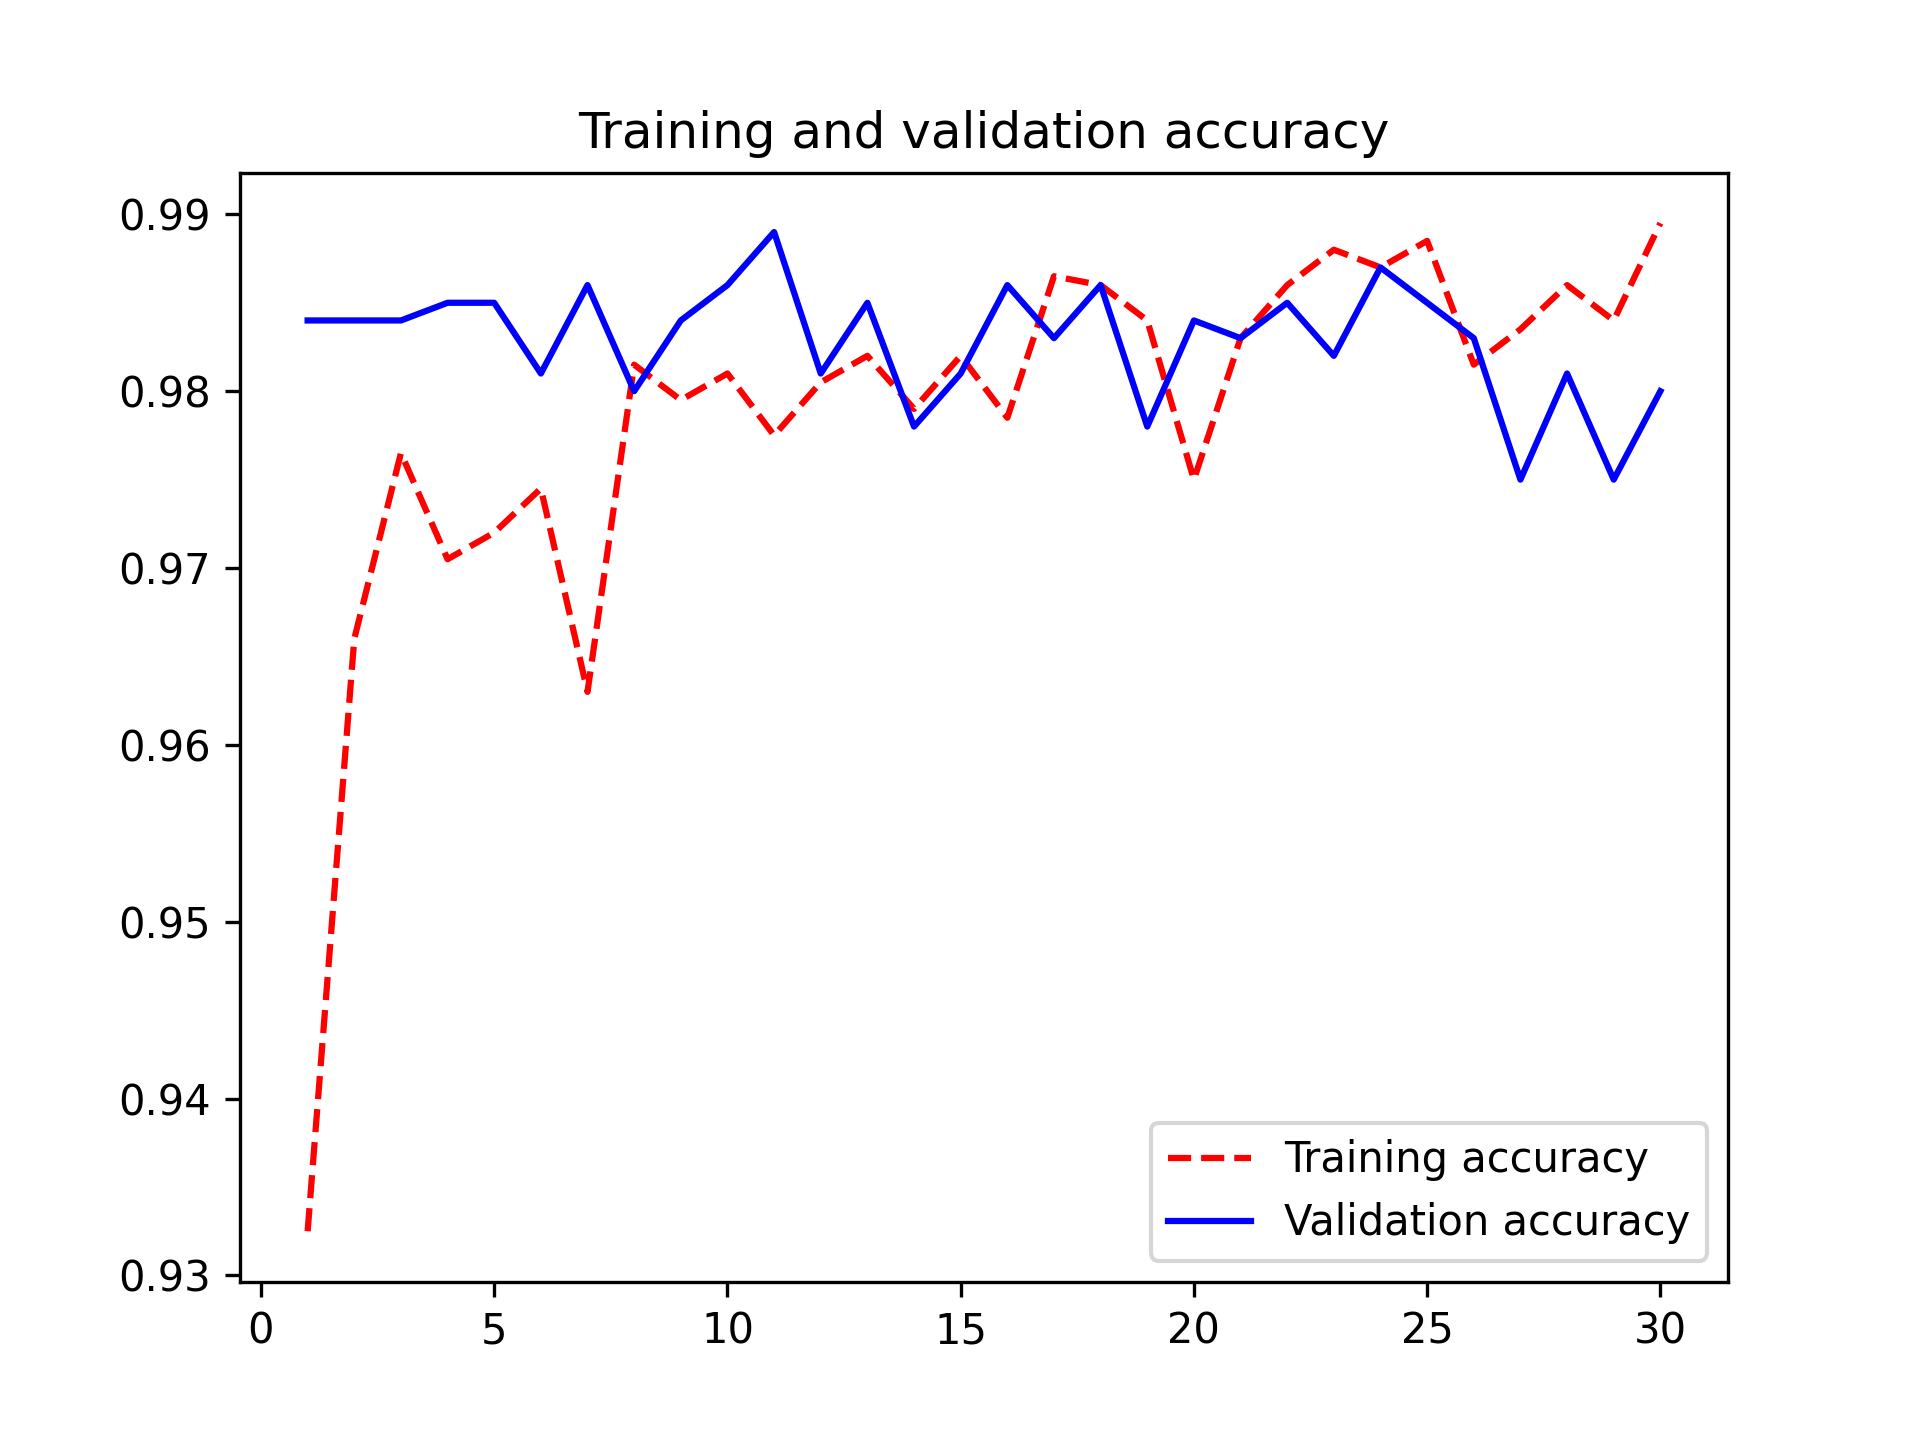
\includegraphics[width=\textwidth,height=0.5\textheight,keepaspectratio]{../../images/ch08/training-and-validation-feda-acc.b0c05268.png}
            \caption{Accuracy FE + Data Augmentation}
        \end{figure}
    \end{columns}
\end{frame}

\begin{frame}{Loss với Feature Extraction + Data Augmentation}
    \begin{columns}
        \column{0.5\textwidth}
        \begin{itemize}
            \item Đồ thị Loss cực kỳ đẹp.
            \item Quá trình này đòi hỏi máy phải có card đồ họa (GPU), vì VGG16 phải chạy dự đoán lại từ đầu qua mỗi bức ảnh biến đổi ngẫu nhiên.
        \end{itemize}
        
        \column{0.5\textwidth}
        \begin{figure}
            \centering
            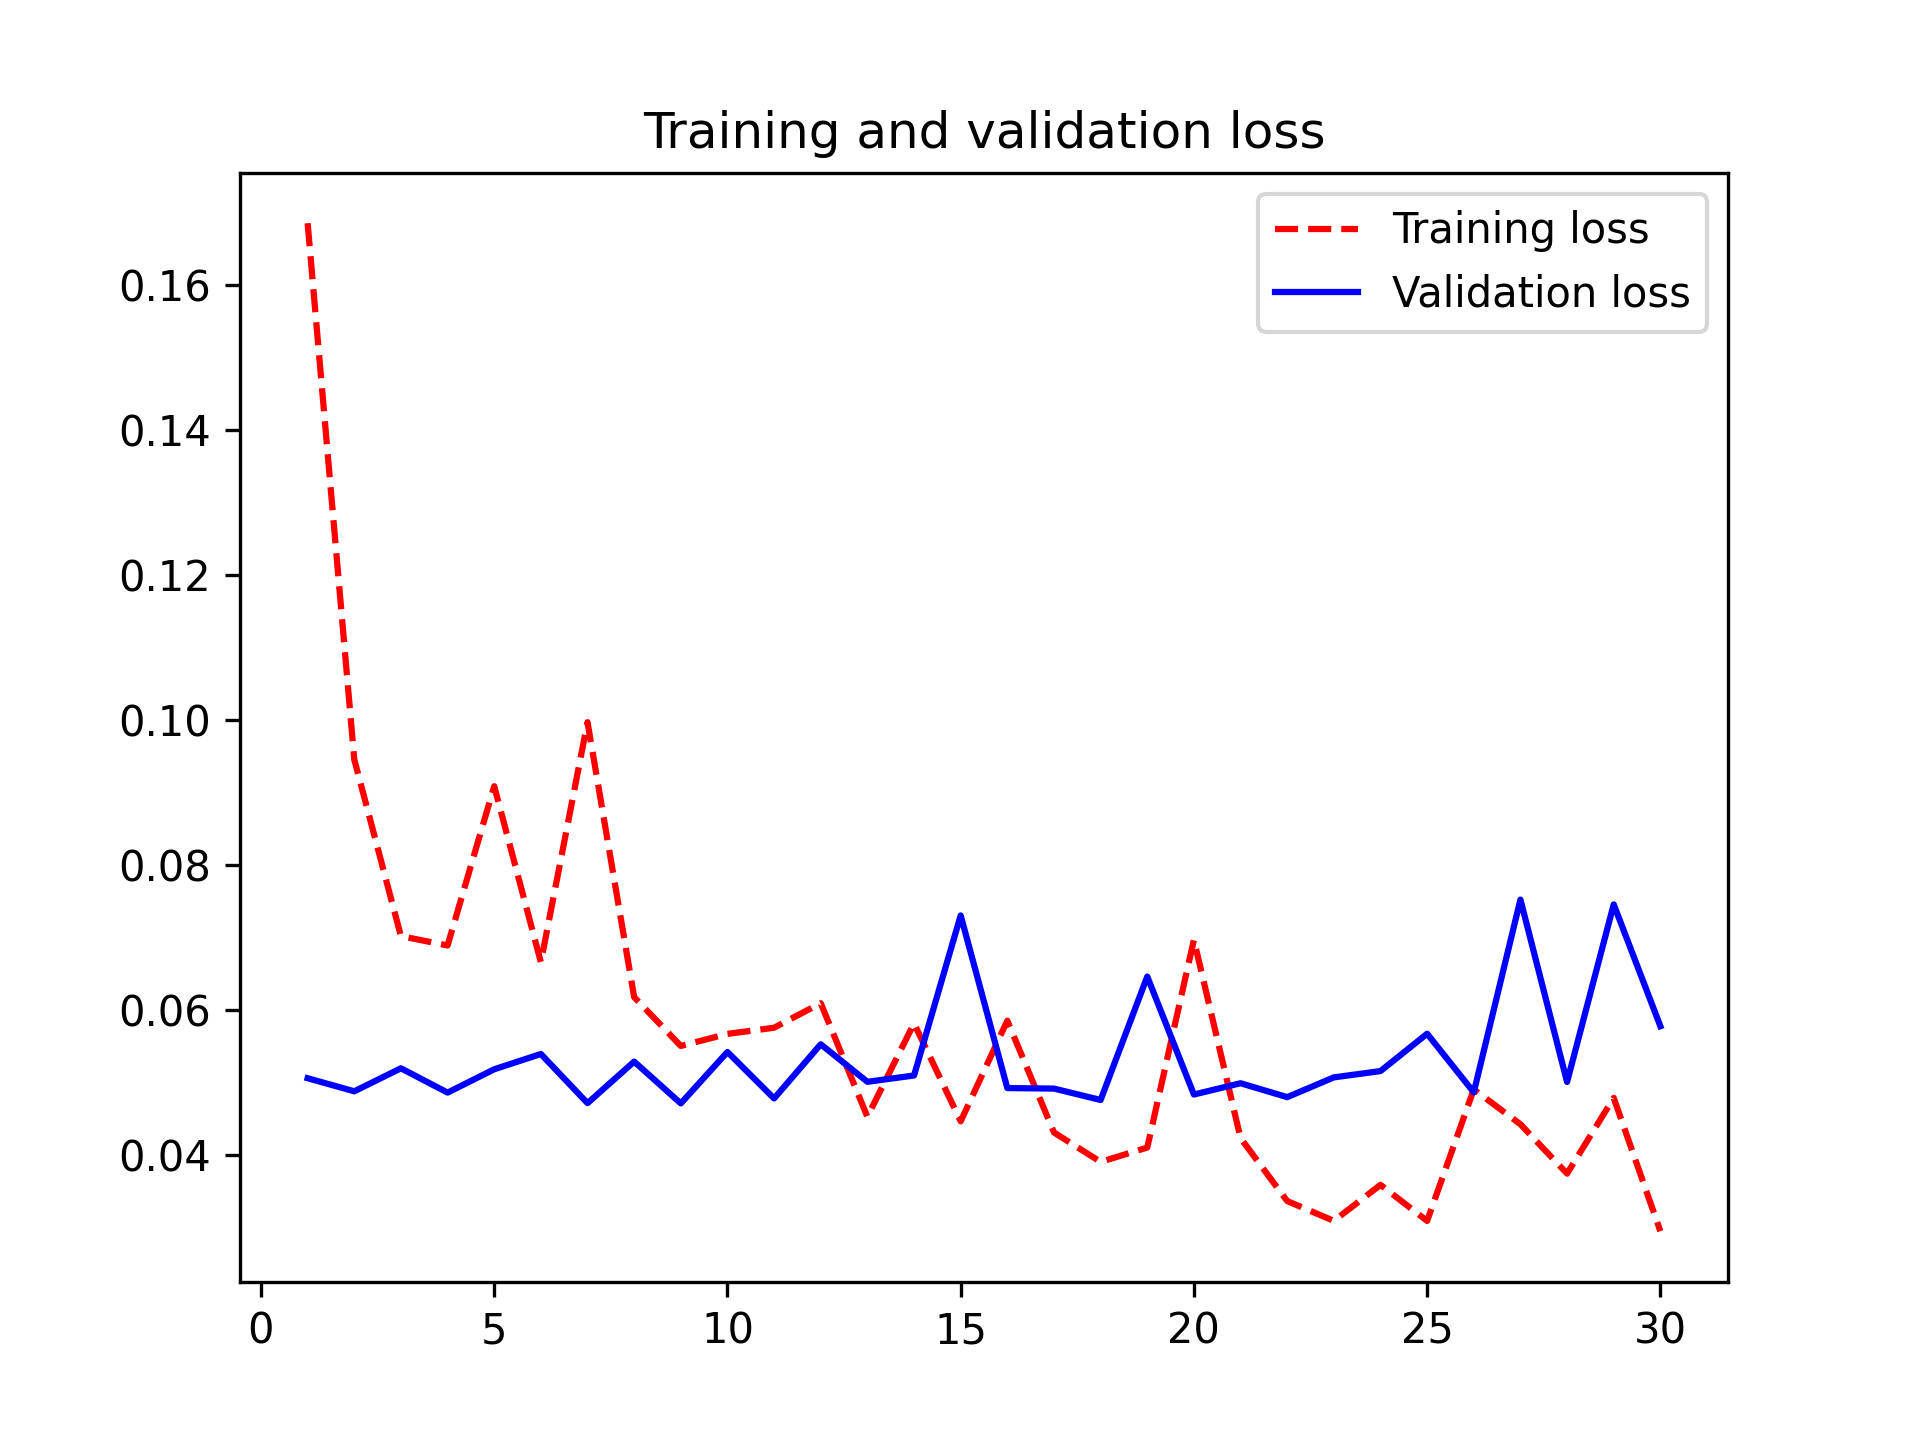
\includegraphics[width=\textwidth,height=0.5\textheight,keepaspectratio]{../../images/ch08/training-and-validation-feda-loss.69d30842.png}
            \caption{Loss FE + Data Augmentation}
        \end{figure}
    \end{columns}
\end{frame}

\section{5. Tinh chỉnh (Fine-Tuning)}

\begin{frame}{Quy trình Fine-Tuning}
    Để ép hiệu suất mô hình đến giới hạn cực đại:
    \begin{enumerate}
        \item Gắn bộ phân loại tùy chỉnh lên trên một mô hình cơ sở (VGG16).
        \item Đóng băng toàn bộ mô hình cơ sở (Freeze Base).
        \item Huấn luyện bộ phân loại tùy chỉnh.
        \item \textbf{Mở khóa (Unfreeze)} một vài lớp Tích chập trên cùng của Base.
        \item Huấn luyện đồng thời cả bộ phân loại và các lớp Tích chập vừa mở khóa với \textbf{Tốc độ học cực nhỏ (Rất nhỏ)}.
    \end{enumerate}
\end{frame}

\begin{frame}[fragile]{Fine-Tuning: Mã nguồn giải mã các lớp cuối}
Chỉ mở khóa Block cuối cùng của VGG16 (block 5).
\begin{lstlisting}[language=Python, basicstyle=\ttfamily\scriptsize]
conv_base.trainable = True

# Freeze all layers EXCEPT the ones from 'block5_conv1' onwards
set_trainable = False
for layer in conv_base.layers:
    if layer.name == "block5_conv1":
        set_trainable = True
    if set_trainable:
        layer.trainable = True
    else:
        layer.trainable = False

# Re-compile model with a VERY SMALL learning rate
model.compile(
    loss="binary_crossentropy",
    optimizer=keras.optimizers.RMSprop(learning_rate=1e-5),
    metrics=["accuracy"]
)
\end{lstlisting}
\end{frame}

\begin{frame}{Kết quả Accuracy sau Fine-Tuning}
    \begin{columns}
        \column{0.5\textwidth}
        \begin{itemize}
            \item Bằng cách nới lỏng nhẹ trọng số của khối Block 5 (VGG16), mô hình tự điều chỉnh các đặc trưng bậc cao sao cho khớp hoàn hảo với chó/mèo.
            \item Độ chính xác vọt lên \textbf{97.5\%}. Đánh bại hoàn toàn mô hình cơ sở ban đầu.
        \end{itemize}
        
        \column{0.5\textwidth}
        \begin{figure}
            \centering
            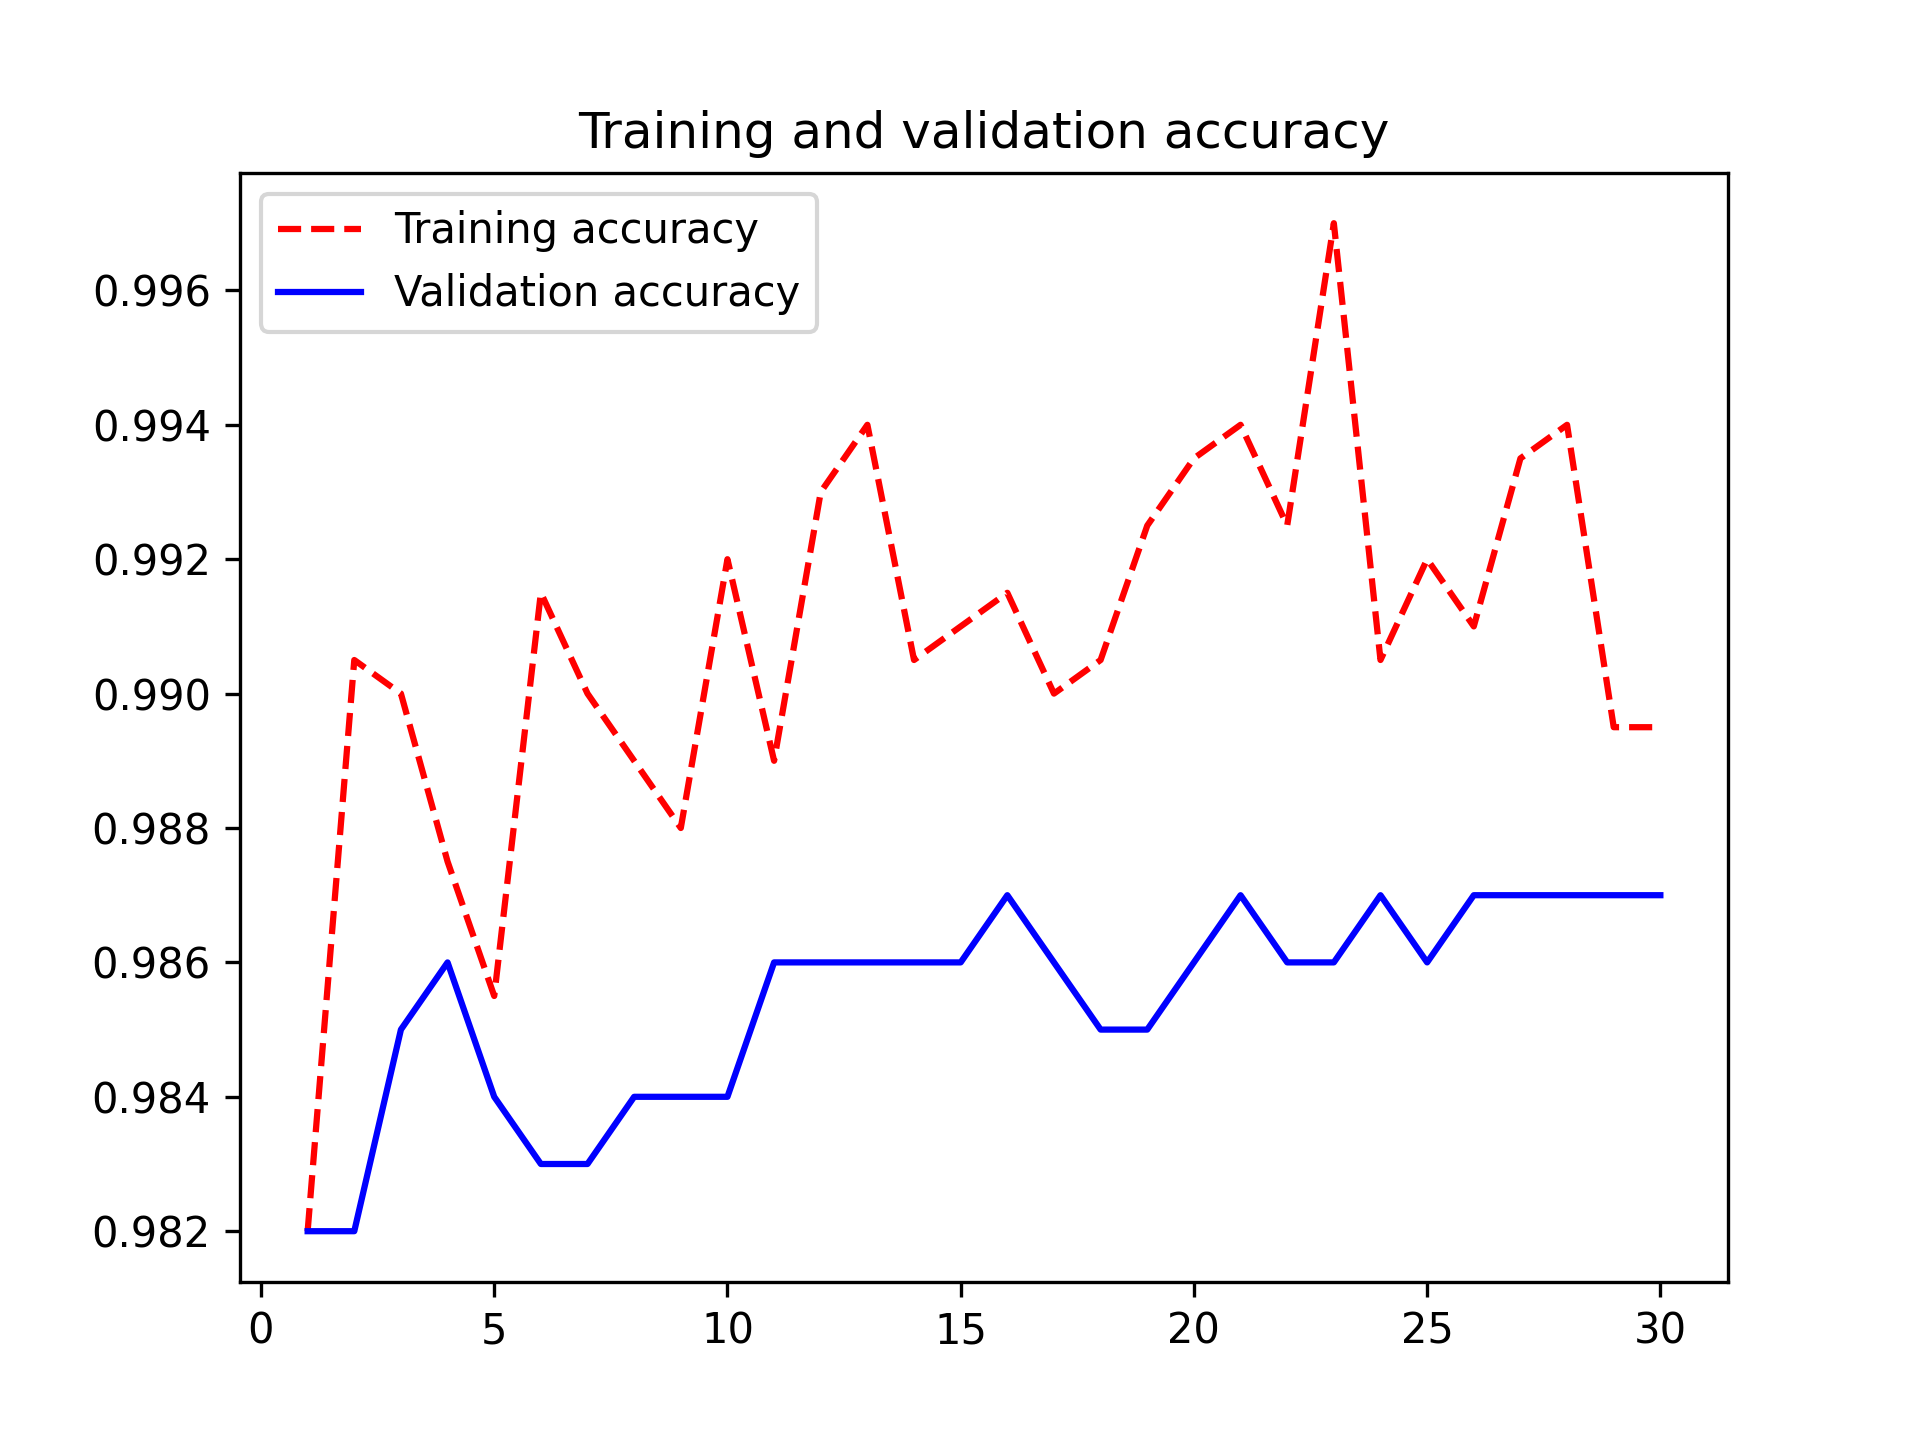
\includegraphics[width=\textwidth,height=0.5\textheight,keepaspectratio]{../../images/ch08/training-and-validation-ft-acc.7ec17959.png}
            \caption{Accuracy sau Fine-Tuning}
        \end{figure}
    \end{columns}
\end{frame}

\begin{frame}{Kết quả Loss sau Fine-Tuning}
    \begin{columns}
        \column{0.5\textwidth}
        \begin{itemize}
            \item Đồ thị Loss có thể biến động nhẹ (nhiễu), nhưng giá trị trung bình trượt dài (Moving Average) cho thấy sự ổn định.
            \item Mặc dù chỉ dùng 2000 ảnh (so với hàng chục ngàn ảnh của người thắng giải Kaggle), ta vẫn đạt kết quả xuất chúng nhờ Transfer Learning.
        \end{itemize}
        
        \column{0.5\textwidth}
        \begin{figure}
            \centering
            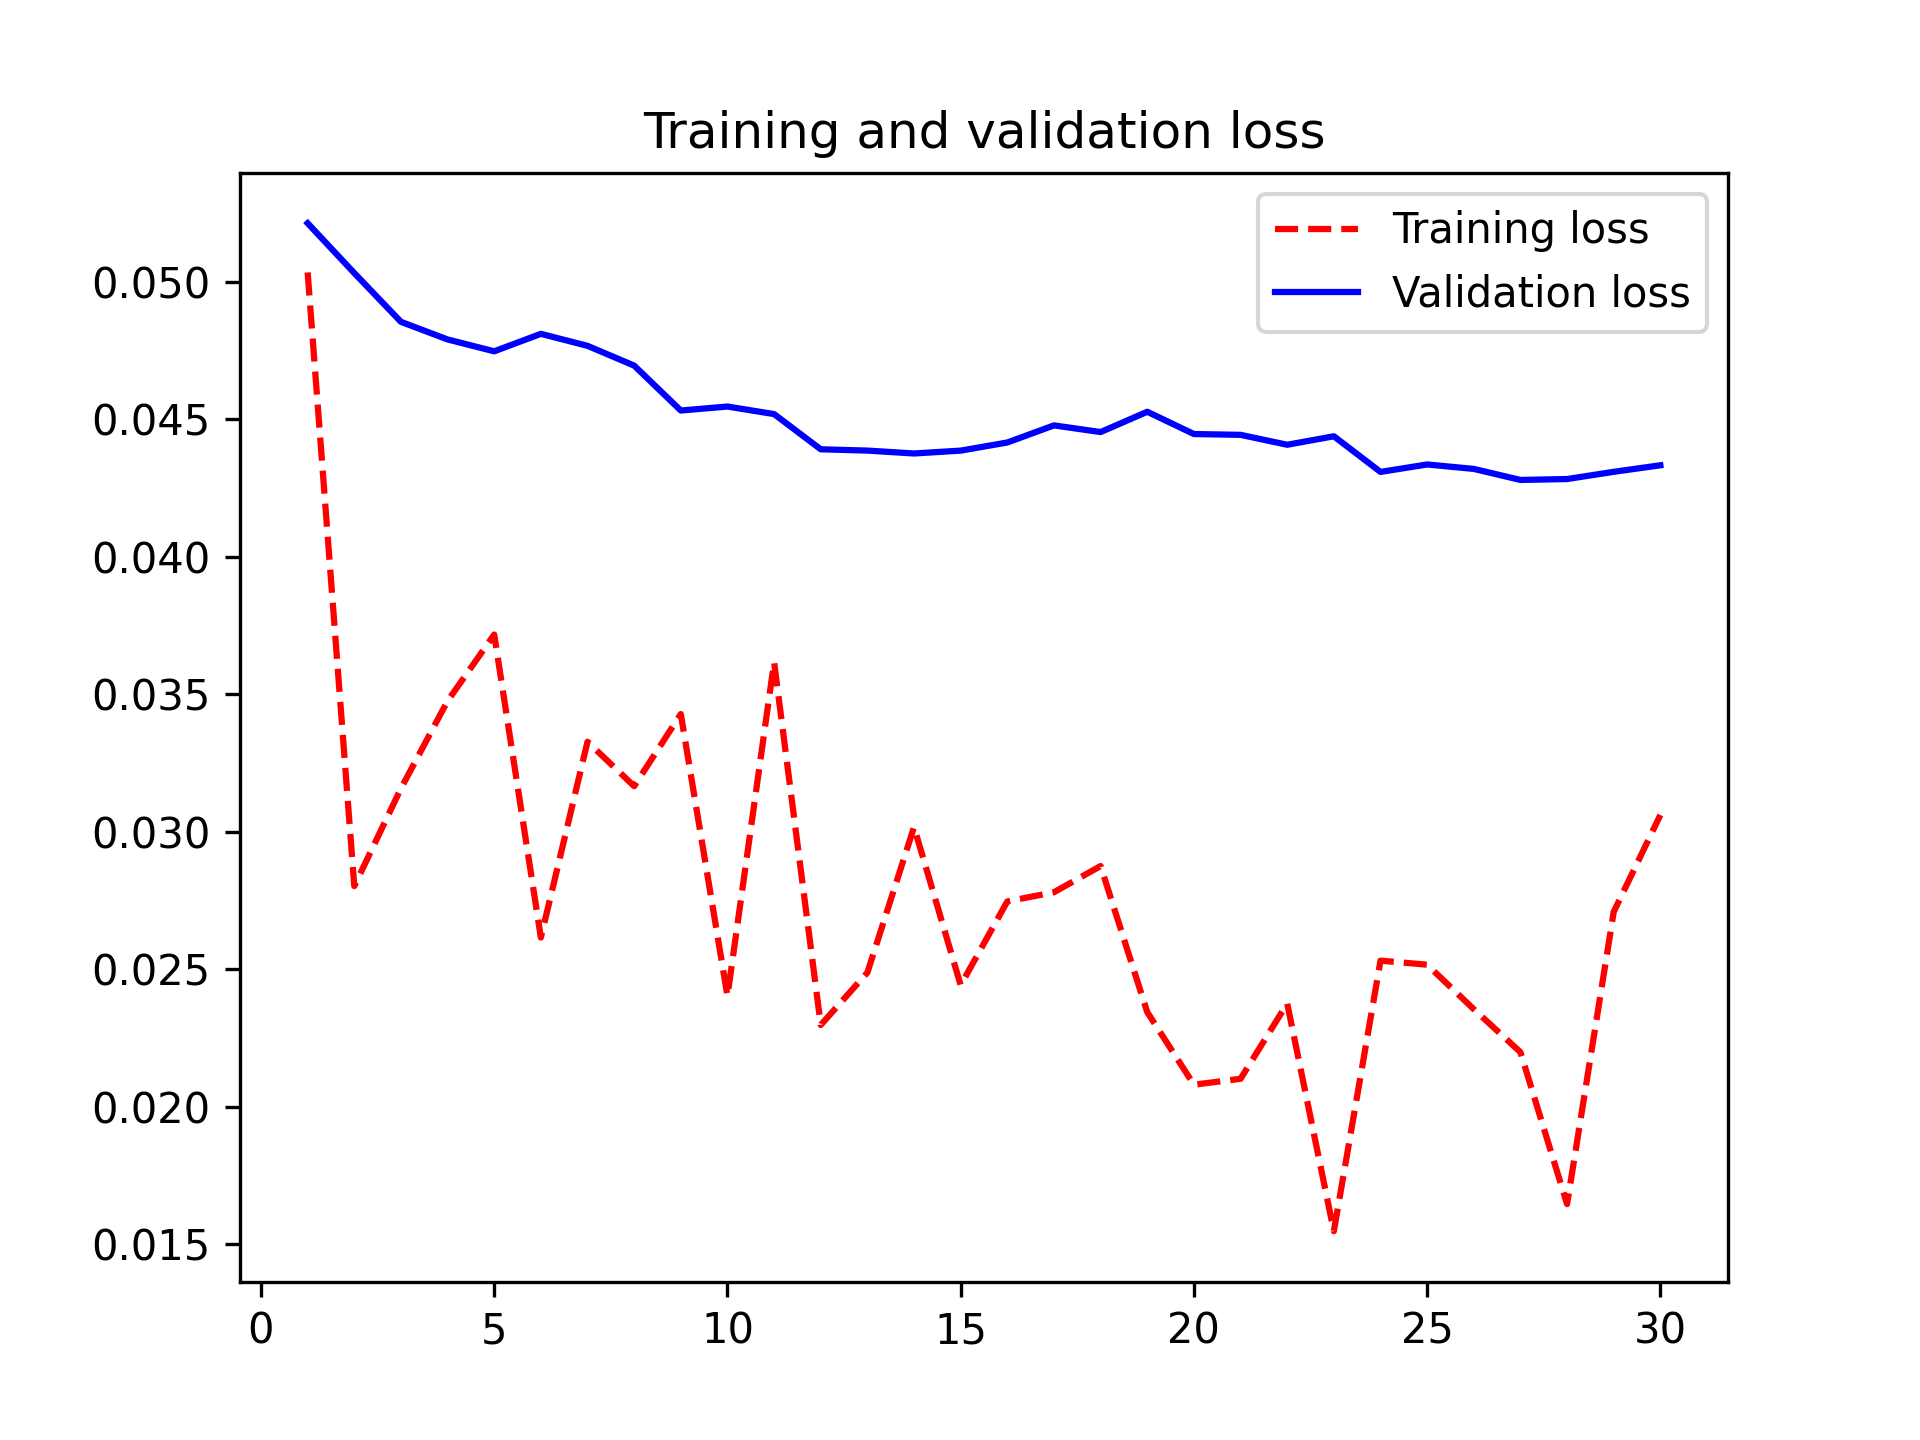
\includegraphics[width=\textwidth,height=0.5\textheight,keepaspectratio]{../../images/ch08/training-and-validation-ft-loss.3c4293eb.png}
            \caption{Loss sau Fine-Tuning}
        \end{figure}
    \end{columns}
\end{frame}

\section{Tổng kết}

\begin{frame}{Tổng kết Chương 8}
    \begin{itemize}
        \item \textbf{Mạng Tích chập (CNN)} vượt trội trong xử lý Ảnh nhờ khả năng học các Mẫu cục bộ bất biến với sự dịch chuyển.
        \item Các khối cơ bản: Phép nhân Tích chập \texttt{Conv2D} và Giảm độ phân giải \texttt{MaxPooling2D}.
        \item \textbf{Data Augmentation} là vũ khí tối thượng chống lại Overfitting khi thiếu hụt Dữ liệu.
        \item Tái sử dụng Tri thức bằng \textbf{Feature Extraction} và \textbf{Fine-Tuning} (VGG16) giúp đạt hiệu suất State-of-the-art chỉ với vài ngàn tấm ảnh.
    \end{itemize}
\end{frame}

\end{document}
